\documentclass[a4paper, doc, floatsintext]{apa6}

\usepackage[english]{babel}
\usepackage{color, soul}
\usepackage{blindtext}
\usepackage{apacite}
\newcommand{\text}{\mbox}
\usepackage{amsmath}
\usepackage{multirow}
\usepackage{setspace}
\usepackage{graphicx}
\usepackage{caption}
\usepackage{subcaption}
\interfootnotelinepenalty=10000



% ---------- watermark -----------
\usepackage[firstpage]{draftwatermark}
\SetWatermarkAngle{0}
\SetWatermarkFontSize{0.25cm}
\SetWatermarkVerCenter{1.15cm}
\SetWatermarkLightness{0.5}
\SetWatermarkHorCenter{14cm}
\SetWatermarkText{\shortstack[l]{
Vong, W. K., Hendrickson, A., Navarro, D. J. and Perfors, A. (2019). Do  \\
additional features help or hurt category learning? The curse of dimensionality \\
in human learners. Cognitive Science, 43, e12724 \\
http://dx.doi.org/10.1111/cogs.12724
}}
\SetWatermarkScale{1}
% -------------------------------

\title{Do additional features help or hurt category learning? The curse of dimensionality in human learners}
\shorttitle{Curse of dimensionality}
\fourauthors{\normalsize Wai Keen Vong}{\normalsize Andrew T. Hendrickson}{\normalsize Danielle J. Navarro}{\normalsize Andrew Perfors}
\fouraffiliations{Department of Mathematics and Computer Science \\ Rutgers University---Newark}{Department of Cognitive Science \& Artificial Intelligence \\ Tilburg University}{School of Psychology \\ University of New South Wales}{School of Psychological Sciences \\ University of Melbourne}

\date{}
\abstract{The curse of dimensionality, which has been widely studied in statistics and machine learning, occurs when additional features causes the size of the feature space to grow so quickly that learning classification rules becomes increasingly difficult. How do people overcome the curse of dimensionality when acquiring real-world categories that have many different features? Here we investigate the possibility that the structure of categories can help. We show that when categories follow a family resemblance structure, people are unaffected by the presence of additional features in learning. However, when categories are based on a single feature, they fall prey to the curse and having additional irrelevant features hurts performance. We compare and contrast these results to three different computational models to show that a model with limited computational capacity best captures human performance across almost all of the conditions in both experiments.}

\newcommand{\wkv}[1]{\textcolor[rgb]{0,0,1}{#1}}


\begin{document}

\maketitle

\section{Introduction}

Despite the fact that category learning is logically difficult in many ways, people easily and naturally learn real-world categories. \citeA{quine60} identified one well-known problem, originating from the fact that the category referent for any particular word is under-determined and could be any from an infinite set of possibilities. This is an example of the problem of induction \cite<e.g.,>{goodman83}, which concerns the difficulty in identifying how to generalize when there are a potentially infinite set of possible bases to do so. The problem of induction, in its different forms, has been widely studied within cognitive science. Proposed solutions often center around the existence of inductive biases, although the exact nature of these biases remains a debated issue \cite<see, e.g.,>{markman89,landauerdumais97,griffithsetal08,goldsmithetal15,minda15}. In this paper, we focus on a less studied but related problem known as the curse of dimensionality. It is similar in that it is a fundamental problem of learnability, but different in that it relates to the specific problem of learning in high-dimensional spaces or with a large number of features. We show why the acquisition of real-world categories \textit{should} be difficult due to the curse of dimensionality, but propose that the structure of real-world categories may alleviate the curse for humans, at least in many situations.

The curse of dimensionality has been well-studied within statistics \cite<e.g.,>{bellman61,donoho00} and machine learning \cite<e.g.,>{verleysenfrancois05,keoghmueen11}, and has a number of interesting and widespread effects. Within computer science, the curse of dimensionality means that if the amount of data on which to train a model (e.g., a classifier) is fixed, then increasing dimensionality can lead to overfitting. This is because as the space grows larger, the examples themselves grow ever sparser; the only way to avoid the issue is to bring in exponentially more data for each additional dimension. In statistics and mathematics, the curse means that it is not possible to numerically optimize functions of many variables by exhaustively searching a discretized search space, thanks to the combinatorial explosion of parameters to explore.

A similar problem arises in the domain of category learning: as we consider categories with more and more features, the size of the possible feature space and number of examples required to fully learn a category grows extraordinarily quickly. For objects with $N$ independent binary features, there are $2^N$ possible examples and $2^{2^N}$ possible ways of grouping these objects into two distinct categories. The number of possible category structures grows at a double-exponential rate, as a function of the number of independent features used to describe stimuli \cite{searcyshafto16}. As a result, even for moderate values for $N$, learning categories should be extremely difficult. For instance, items with 16 possible features of two possible values each yields $65 536$ possible exemplars.

% If features can take on more than two values -- as in most real-world categories -- the problem grows even more acute.


Most real-world categories have a large number of available features for categorization \cite{rosch1973natural}, which suggests that -- in theory at least -- the curse of dimensionality means that acquiring natural categories should be a difficult learning problem. Yet people, including children, can learn real-world categories with relative ease, often based on only a few exemplars. How do people accomplish this feat?

We know surprisingly little about the answer to this question. Most experimental work in category learning has not run into the problem of the curse of dimensionality, either because studies have used categories that people have already learned or because they tested categories using stimuli with only a few, highly salient features \cite<e.g,>{shepard1961learning, medin1978context, nosofsky1986attention}. Although this body of work has substantially contributed to our understanding of category learning, it remains an open question how learning is affected when there are a large number of features.

While some studies in the category learning literature have used stimuli with a large number of features \cite<e.g,>{mclaren1994recognition,wills1997generalization, wills1998perceptual,jones1998perceptual}, the focus of these particular studies was not directly related to how varying the number of features impacts learning. Furthermore, the limited set of studies that have investigated category learning with varying numbers of features have yielded conflicting results, with some studies finding that additional features impair learning \cite{edgell1996irrelevant}, others finding that they facilitate learning \cite{hoffman2006category,hoffman2008prior}, and others finding that they have no effect on learning at all \cite{minda2001prototypes}, or that they do both \cite{bourne1959mathematical}.

How can we resolve this apparent discrepancy? One possibility is that each of these studies differ in the kinds of category structures being learned. After all, the curse of dimensionality stems from having so many possible stimuli configurations in a high-dimensional space that it is difficult to learn which set of features people should use for classification. This should lead to the greatest inefficiency when most of the possible features are not predictive of category membership and only one or a few matter, as in \citeA{walker1961identification} and \citeA{edgell1996irrelevant}. By contrast, if all features are predictive to some degree -- especially if they are not perfectly correlated with each other -- then additional features should be beneficial, or at least not harmful  \cite{hoffman2006category,hoffman2008prior,minda2001prototypes}. This possibility is especially interesting given the fact that most real-world categories have precisely this sort of family resemblance structure \cite{roschmervis75,murphy02}.

This hypothesis -- that a family resemblance category structure may mitigate the impact of the curse of dimensionality, but that other kinds of category structures may not -- appears plausible on its face, but to date no studies have tested it. The goal of the current paper is to examine this hypothesis by manipulating category structure and the number of features while holding other factors constant. Our results do indeed suggest that people do not succumb to the curse if the categories follow a family resemblance structure. However, if only a single feature is relevant among a set of features for categorization, the curse of dimensionality affects humans. We argue that the pattern of performance reflects capacity limitations that prevent people from learning from and using more than a few features at a time. As a result, learning is impaired where only one or a few features are predictive, but it is not affected when many different features are all predictive (as any given feature will be similarly useful). We support this interpretation by a comparison of several computational models with different assumptions about representation and capacity limitations, and we find that human performance is best fit by a model with limited capacity for learning.

% WK: previous version based on optimal model
% We compare these results to an ideal observer model for this task that shows the theoretical accuracy one could achieve by combining information across all of the available features. Despite human performance falling well below the achievable limit given by this ideal observer model, our results show that there are situations in which people can still achieve high classification performance and overcome the curse of dimensionality.

\section{Experiment 1}

We addressed two questions in this experiment. First, how does learning performance change as the number of features increase? Second, to what extent does the structure of the category influence this learning? We therefore systematically manipulated the number of features and the manner in which categories were structured within the context of a standard supervised learning task.

\subsection{Method}

\subsubsection{Participants}
886 participants (496 male, 388 female, 2 other) were recruited via Amazon Mechanical Turk. This is a relatively high number of participants because we ran two experiments with slightly different methodologies (described below) but pooled the results since they were qualitatively identical. Participants ranged in age 18 to 76 (mean 34.2). They were paid US\$2.00 for completion of the experiment, which took roughly 12 minutes. Data from an additional 42 participants were excluded from analysis, either from failure to complete the task (37 participants) or participating in a pilot version of the study (5 participants).

\begin{figure}[t]
  \begin{center}
    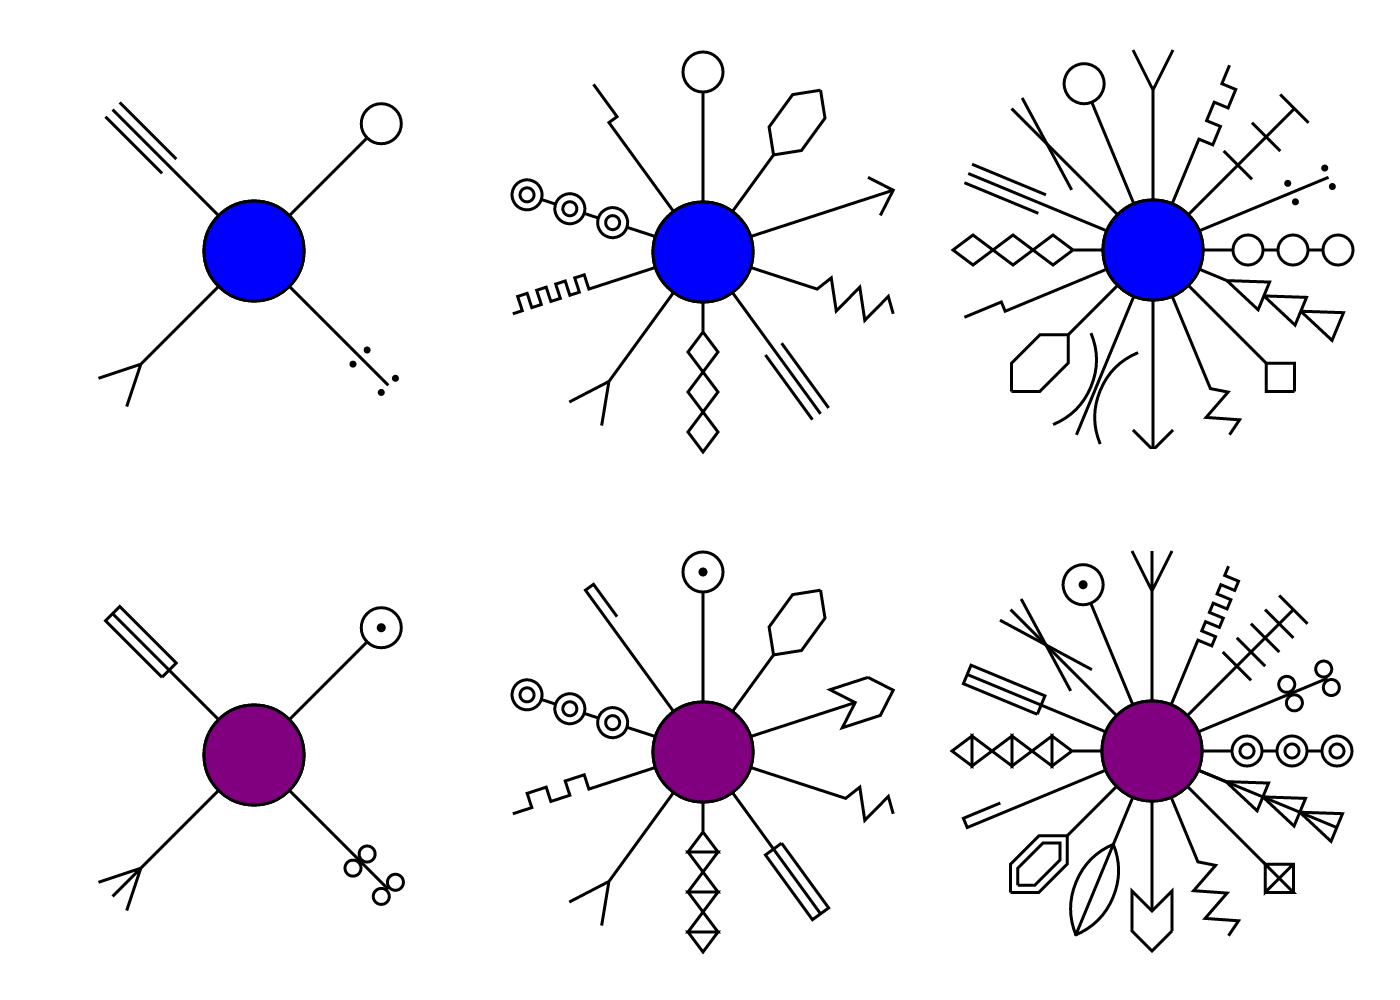
\includegraphics[width=0.8\textwidth]{figures/stimuli.png}
    \caption{\small{Example stimuli, displaying two instances from each of the three possible \textit{Dimensionality} conditions (4, 10, and 16, from left to right). Features were binary and correspond to the legs of the amoebas. Together, the two 16-\textsc{feature} examples show all possible feature values.}}
    \label{experiment-stimuli}
          \vspace{-5mm}
  \end{center}
\end{figure}

\subsubsection{Design}

The experiment presented people with a supervised category learning problem, in which they were asked to classify an amoeba stimulus as either a \textsf{bivimia} or \textsf{lorifen}. Each amoeba consisted of a circular base with a set of binary features (legs). The full set of 16 unique pairs of features are shown on the two stimuli in the right column of Figure~\ref{experiment-stimuli}.

Nine experimental conditions were created by manipulating the \textit{Dimensionality} of the stimuli and the \textit{Structure} of the category in a 3 $\times$ 3 between-participants design; people were randomly assigned to each condition. The three levels of \textit{Dimensionality} reflect the number of binary features present on the stimuli: 4-\textsc{feature} ($N$ = 302), 10-\textsc{feature} ($N$ = 277), or 16-\textsc{feature} ($N$ = 307). For the lower-dimensionality conditions, the set of displayed features were a randomly selected subset of the features used in the 16-\textsc{feature} condition. The position of features on the amoeba were randomized differently for each participant.

The three category \textit{Structures} were designed in the following way. In every condition there was one feature (chosen randomly) that was 90\% predictive of the category label, such that 90\% accuracy could be achieved by using that feature alone. However, the predictiveness of the other features differed as a function of \textit{Structure} condition. In the \textsc{single} condition ($N$ = 294), all other features were completely non-predictive (i.e., the value of that feature predicted a given label 50\% of the time). As such, the best performance in the \textsc{single} condition would be achieved by identifying the single predictive feature and making categorization decisions using only it. By contrast, in the \textsc{all} condition ($N$ = 301), all of the features were 90\% predictive, matching a family resemblance structure. As a consequence the best possible performance is achievable by aggregating the information provided by all features. Finally, in the \textsc{intermediate} condition ($N$ = 291), the other features were 70\% predictive. Thus, one feature was most diagnostic but it would be theoretically possible to achieve better performance by using all of the features in concert. By using features that are 90\% predictive, rather than 100\% predictive of category membership, allows us to disambiguate between whether people are using a single feature, or multiple features, when classifying stimuli with many features across the three \textit{Structure} conditions.

\subsubsection{Procedure}

\begin{figure}[t]
  \begin{center}
    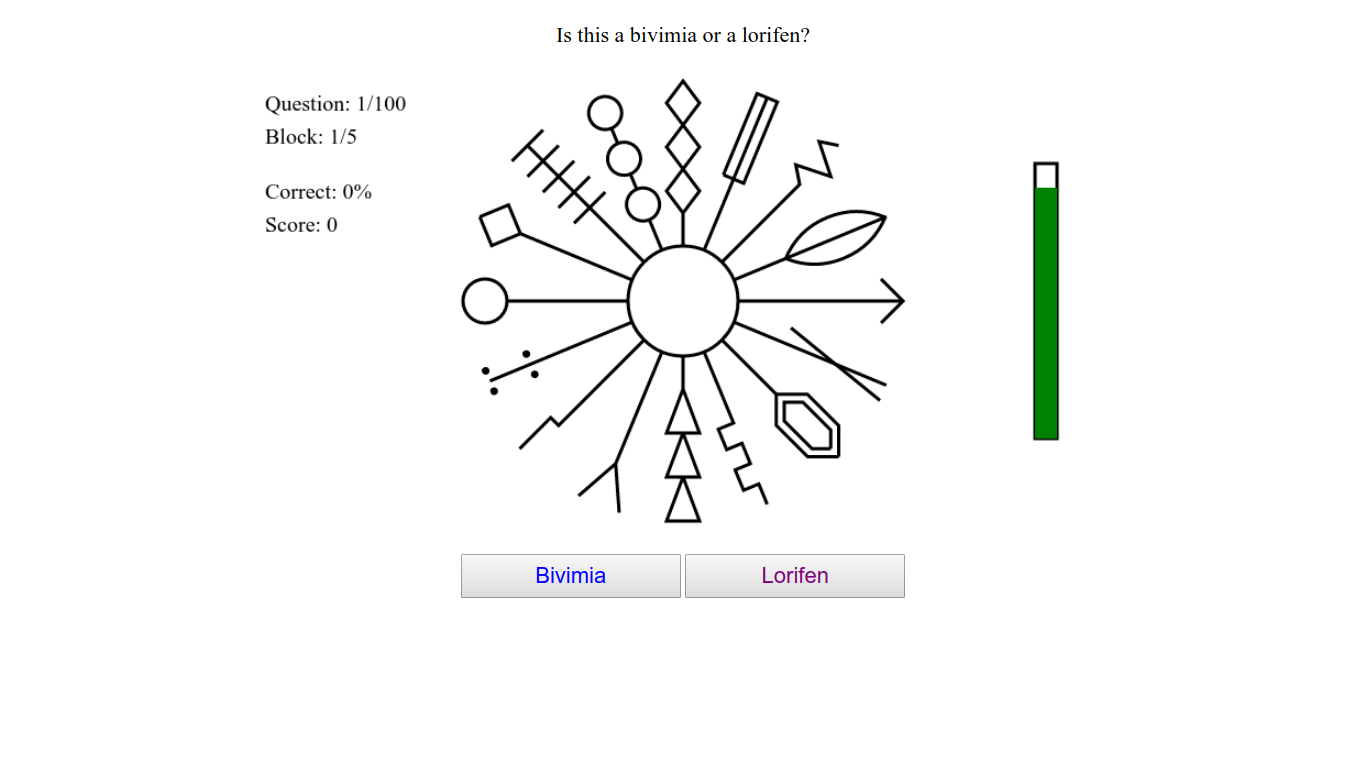
\includegraphics[width=0.9\textwidth]{figures/experiment-trial.png}
    \vspace{-10mm}
    \caption{{\small An example of a trial from the 16-\textsc{feature} condition. Participants were asked to classify the amoeba as either a \textsf{bivimia} or a \textsf{lorifen}. In one version of the experiment, a green timer on the right was displayed to incentivize participants to respond faster for additional points, which they were given for correct answers only. Another version of the experiment was also run that did not include the timer.}}
    \label{experiment-trial}
          \vspace{-5mm}
  \end{center}
\end{figure}

The experiment consisted of five blocks of 20 learning trials each, resulting in a total of 100 trials. During the instructions at the beginning of the experiment, participants were presented with a randomly selected example stimuli that was unlabeled to give them a preview of the kinds of objects they would be learning to categorize. On each trial people were presented with an amoeba as shown in Figure \ref{experiment-trial} and were instructed to classify it as either a \textsf{bivimia} or a \textsf{lorifen}.\footnote{In all conditions, the stimuli were generated probabilistically and independently of one another, rather than pre-generating 100 specific stimuli and showing the same ones to everybody. To perform this, one of the two categories was randomly selected on each trial, and then the features of the stimulus were generated according to the conditional probabilities based on the category structure for that condition.} People received points for correct answers but did not lose points for incorrect ones. In one version of the experiment ($N$ = 439) people were given as much time as they wanted to respond; in the other ($N$ = 447), they were still given as much time as they liked but they saw a timer (the green bar on the right of Figure~\ref{experiment-trial}) that slowly decreased, and they received more points for faster answers. There were no differences in performance between these two versions so the data was pooled and results reported are from the combined dataset\footnote{For the main analyses reported in this paper, we performed a model comparison between a model with \textsc{timer} as an additional discrete predictor and model without. Results from this model comparison for both experiments produced Bayes factors that favoured the models which did not include an effect for \textsc{timer}. This suggested that the presence or absence of the timer had little effect on participant's accuracy in the task, so it was sensible to pool the data into a single dataset.}.

Participants were given feedback which was displayed for three seconds. It consisted of a \textsf{correct} or \textsf{incorrect} message, the number of points earned, the correct category label, and a change to the color of the circular base of the amoeba to indicate category membership (blue for \textsf{bivimias} and purple for \textsf{lorifens}). Before the next trial was displayed, a blank screen was shown for one second. At the end of each block of 20 trials, people were given a short summary of their performance, showing them their accuracy and points earned in the current block and all previous blocks.

\subsection{Results}

\begin{figure}[t]
  \begin{center}
    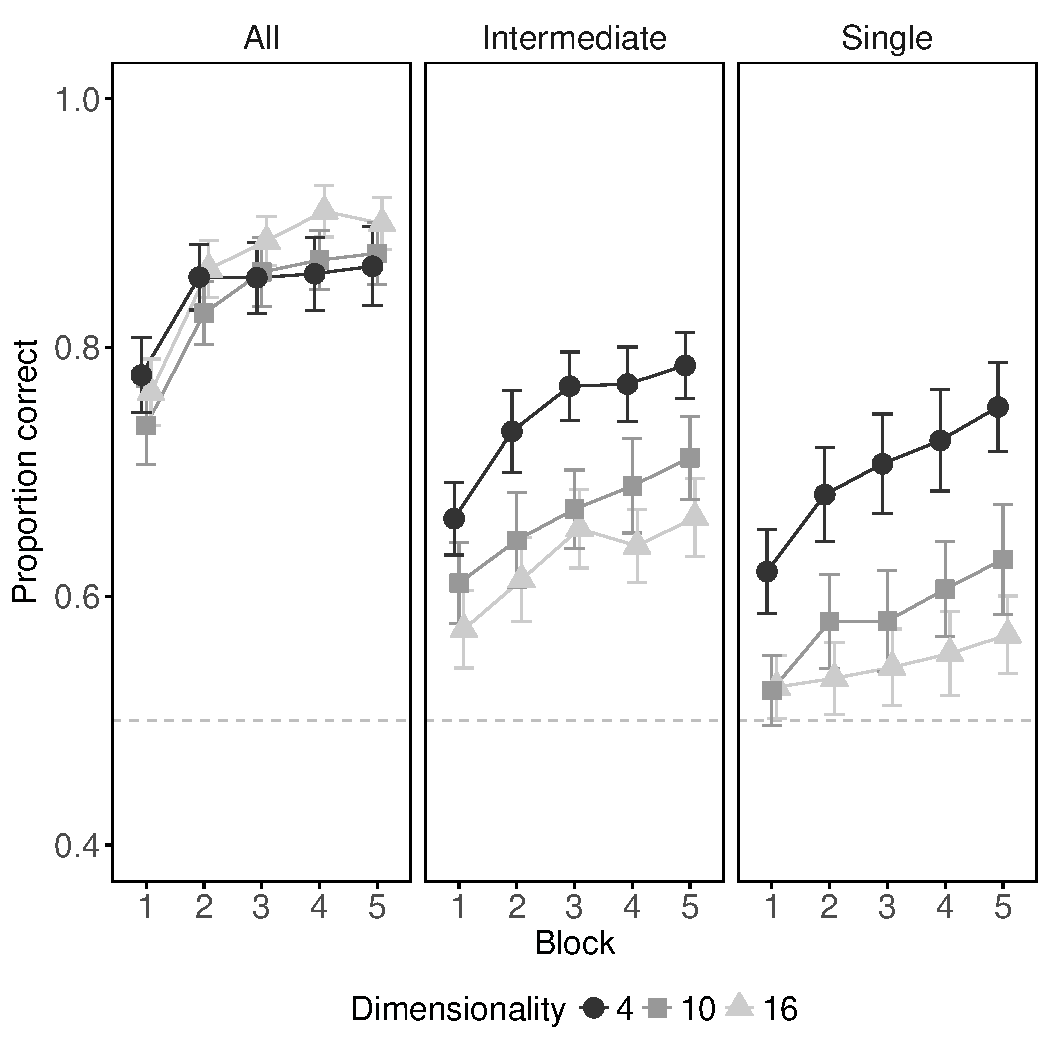
\includegraphics[width=0.75\textwidth]{figures/mean-performance-experiment-one.pdf}
    \caption{\small{\textbf{Accuracy in Experiment 1}. Human learning across the \textit{Dimensionality} and \textit{Structure} conditions. While learning within the \textsc{all} condition was unaffected by the number of features, more features led to poorer performance in the \textsc{single} and \textsc{intermediate} categories. Error bars depict 95\% confidence intervals, and the dotted line reflects chance performance.}}
    \label{mean-performance-experiment-one}
  \end{center}
      \vspace{-5mm}
\end{figure}

Participants learned well in all conditions, with accuracy increasing across training block (Figure~\ref{mean-performance-experiment-one}). We quantified this effect through the use of Bayesian mixed effects model comparison in which we compared a baseline model that contains only a random intercept for each participant to a model that includes a linear effect of \textit{Block}.\footnote{All mixed effects models in this paper assume a random intercept for each subject. Bayes factors were calculated using the default parameters \cite{rouder2012default,liang2012mixtures} of the BayesFactor package 0.9.12-2 \cite{bayesfactor} in R 3.2.3.} The Bayes factor for this comparison ($BF > 10^{77} : 1$) overwhelmingly favors the model that includes an effect of \textit{Block}. The posterior estimate of block shows a positive slope of 0.025 (95\% CI is 0.022 to 0.027) indicating that average accuracy increased by about 2.5\% for each block of training.

While it is reassuring that there is a general improvement in accuracy throughout training, one of our main questions was whether accuracy differed as a function of category \textit{Structure}. Figure~\ref{mean-performance-experiment-one} suggests two things: first, that accuracy in the \textsc{all} structure is much higher than the \textsc{intermediate} and \textsc{single} category structures; and second, that the learning rate may be identical across all category structures. To investigate the first issue, we evaluated whether there was an effect of \textit{Structure} on accuracy. Indeed, a model with two predictors (\textit{Structure}, coded as a three-level categorical variable, and \textit{Block}) is strongly preferred over a model containing only \textit{Block} ($BF > 10^{90} : 1$). Posterior estimates reveal that accuracy in the \textsc{all} condition is 0.16 higher (95\% CI is 0.12 to 0.20) than the \textsc{intermediate} structure, which is slightly higher than the \textsc{single} (0.08 more, 95\% CI from 0.04 to 0.12). In order to investigate the second issue, we compared the \textit{Structure} and \textit{Block} model to a more complex model that also included an interaction between \textit{Structure} and \textit{Block}. The model without an interaction is strongly preferred ($BF = 40 : 1$), suggesting that the rate of learning across blocks is not different in the three \textit{Structure} conditions.

Our second question was whether there is evidence for an effect of stimulus \textit{Dimensionality} on performance. We found that there was: a model containing \textit{Dimensionality} (coded as a three-level categorical variable) and \textit{Block} was strongly preferred over a model containing only \textit{Block} ($BF > 10^{7} : 1$). The posterior estimates of the effect of number of dimensions show that there were reliable differences was between the 4-\textsc{feature} condition versus the 16-\textsc{feature} and 10-\textsc{feature} conditions. The estimates showed that the 4-\textsc{feature} was on average 0.08 more accurate than the 16-\textsc{feature} condition (95\% CI is 0.03 to 0.13), and 0.05 more accurate than the 10-\textsc{feature} condition (95\% CI is 0.01 to 0.10). No difference was observed between the 10-\textsc{feature} and 16-\textsc{feature} conditions.

Of course, we are less interested in whether dimensionality or category structure \textit{alone} has an effect on learning, and most interested in whether there is an interaction: do more stimulus dimensions, as hypothesized, hurt learning in the \textsc{single} category structures but not in the \textsc{all} category structures? To evaluate this, we compared a Bayesian mixed effects model containing \textit{Block}, \textit{Structure}, and \textit{Dimensionality} alone to a model with these three variables plus an interaction term between \textit{Structure} and \textit{Dimensionality}. This shows strong evidence in favor of the model containing the interaction ($BF > 10^{8} : 1$), indicating that additional features have different effects on learning in different category structures.

\begin{table}[t]
\centering
\label{my-label}
\begin{tabular}{cccc}
\toprule
 & All                          & Intermediate                   & Single                           \\ \midrule
Bayes factor       & 0.3:1                             & $\mathbf{10^{8}:1}$                     & $\mathbf{10^{11}:1}$                     \\
4 vs. 10           & 0.01 (-0.05 to 0.07)    & \textbf{0.08 (0.01 to 0.14)}  & \textbf{0.11 (0.04 to 0.18)}  \\
10 vs. 16          & -0.03 (-0.09 to 0.03) & 0.04 (-0.03 to 0.10) & 0.03 (-0.03 to 0.10) \\
4 vs. 16           & -0.02 (-0.08 to 0.04)  & \textbf{0.11 (0.05 to 0.17)} & \textbf{0.15 (0.07 to 0.22)} \\ \bottomrule
\end{tabular}
\vspace{2mm}
\caption{\small{Bayes factors and parameter estimates for the post-hoc analyses of the effect of stimulus \textit{Dimensionality} for each category \textit{Structure} in Experiment 1. The first row indicates the Bayes factor in favour of a model with Dimensionality and Block as predictors relative to a model with only Block; all other rows show the posterior estimates of the differences between Dimensionality conditions within that category structure. Results indicate that the effect of stimulus dimensionality was larger in the \textsc{single} and \textsc{intermediate} than the \textsc{all} category structure. The 95\% confidence interval estimates are shown inside the brackets.}}
\label{exp1-post-hoc-table}
\end{table}

What differences drive this interaction? Figure~\ref{mean-performance-experiment-one} suggests that accuracy in the \textsc{intermediate} and \textsc{single} category structure conditions decreases much more strongly as the number of stimulus features increases. In order to investigate this quantitatively, we conducted a post-hoc analysis of the effect of \textit{Dimensionality} on accuracy within each category structure. The results, shown in Table~\ref{exp1-post-hoc-table}, indicate the Bayes factor in favor of a mixed effects model containing \textit{Dimensionality} and \textit{Block} relative to a model containing only \textit{Block}. The results show that for the \textsc{intermediate} and \textsc{single} structures, the model with the higher Bayes factor includes the \textit{Dimensionality predictor}, suggesting that the number of features affects learning for these structures. However, for the \textsc{all} structure the preferred model based on its Bayes factor is one without \textit{Dimensionality} as a predictor. This is consistent with our hypothesis that additional features should hurt learning much more strongly when categories do not follow a family resemblance structure.

\subsection{Summary}

Experiment 1 suggests that increasing the number of features has a differential impact depending on the underlying category structure. In the two conditions that contain a single highly predictive feature and other features that are less predictive (\textsc{single} and \textsc{intermediate}), learning is clearly improved when there are fewer features overall. This is most evident in the final two columns of Table~\ref{exp1-post-hoc-table}, which show 10-14\% increases in overall accuracy for learning from four rather than 16 features in the \textsc{intermediate} and \textsc{single} conditions. The same advantage does not occur in the \textsc{all} category structure .

The fact that learning was not impaired in the \textsc{all} category structure may not be particularly surprising, given that all features were equally useful and there were no features that were less predictive. In that sense it is the lack of \textit{advantage} for more features that is perhaps more surprising, especially since other studies have shown a learning advantage when there are additional features \cite<e.g.,>{hoffman2006category, hoffman2008prior}. One possibility here is that performance in the \textsc{all} condition reflects a ceiling effect. Since all of the features were 90\% predictive, it could be that the task was quite easy no matter how many features there were. We test this directly in Experiment 2 by investigating only family resemblance structures, but manipulating the degree to which the features are predictive of the category label.

\section{Experiment 2}

This experiment explicitly tests whether additional features have an effect on category learning within family resemblance categories when the features are less predictive than in the previous experiment. If there is no effect of the number of features on learning, we can be more certain that the differences due to category structure found in Experiment 1 are actually due to category structure rather than to the informativeness of the features. We test this by systematically manipulating the predictiveness of the features. Does this affect the degree to which additional features affect learning?

\subsection{Method}

\subsubsection{Participants}

888 people (459 male, 425 female, 4 other) were recruited via Amazon Mechanical Turk. As before, the high number of participants reflects the fact that we ran two experiments with slightly different methodologies and pooled the results since they were qualitatively identical ($N$ = 436 for the version without the timer, $N$ = 452 for the version with it). Participants ranged in age from 19 to 74 (mean 34.6). They were paid US\$2.00 for completion of the task, which took 12 minutes. Data from an additional 37 participants were excluded from analysis, either from failure to complete the task (32 participants) or participating in an earlier version of this study (5 participants).

\subsubsection{Design}

The task and stimuli were identical to Experiment 1, with participants randomly allocated in a 3 $\times$ 3 between-participants design. As before, we manipulated the \textit{Dimensionality} by altering the number of features present in the stimuli to make three conditions: 4-\textsc{feature} ($N$=286), 10-\textsc{feature} ($N$=327), and 16-\textsc{feature} ($N$=275). Unlike before, all the category structures were family resemblance structures, with all features being equally predictive of the category. This time we manipulated the degree of \textit{Predictiveness} to make three conditions: 70\% predictive ($N$=310), 80\% predictive ($N$=258), and 90\% predictive ($N$=320). The 90\% condition was a replication of the \textsc{all} structure in Experiment 1.

\subsubsection{Procedure}

The procedure was identical to Experiment 1. Similar to the previous experiment, in one version of the experiment ($N$ = 436), there was no time limit for providing a response on each trial. In the other version of the experiment ($N$ = 452), there was still no time limit, but they saw a timer that slowly decreased (see Figure~\ref{experiment-trial}), and they received more points for faster responses.

\subsection{Results}

\begin{figure}[th!]
  \begin{center}
    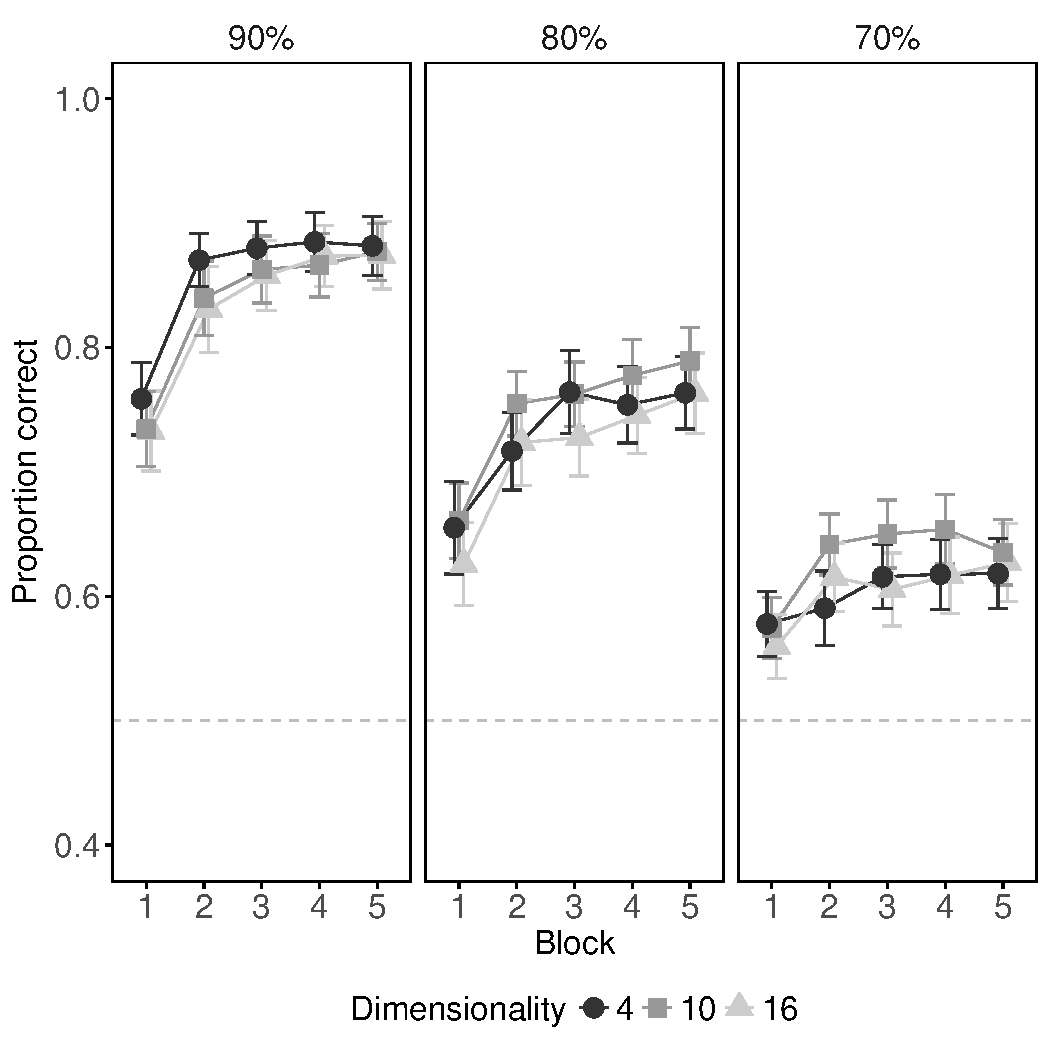
\includegraphics[width=0.75\textwidth]{figures/mean-performance-experiment-two.pdf}
    \caption{\small{\textbf{Results from Experiment 2}. Mean accuracy across the three \textit{Predictiveness} and \textit{Dimensionality} conditions. While the mean performance decreased as the level of \textit{Predictiveness} was reduced, within each \textit{Predictiveness} condition there was no change based on the number of features. Error bars show 95\% confidence intervals, and the dotted line reflects chance performance.}}
    \label{mean-performance-experiment-two}
  \end{center}
\end{figure}

How was learning affected by \textit{Dimensionality} and \textit{Predictiveness}? We evaluated this question by comparing Bayesian mixed effects models that included some combination of \textit{Block} as a continuous variable and \textit{Dimensionality} and \textit{Predictiveness} as discrete variables. Reassuringly, we found that people did indeed learn over the course of training: a model including \textit{Block} was strongly preferred over a model that only contained a random effect for each participant (\textit{BF} > \(10^{74}\):1). As before, posterior estimates suggest that average accuracy increased by about 2.3\% for each block of training (95\% CI is 0.020 to 0.025).

How did the \textit{Predictiveness} of features affect learning? As Figure \ref{mean-performance-experiment-two} shows, and as one would expect, overall learning was lower in categories with lower predictiveness. This is borne out in a Bayesian model comparison between a model with \textit{Predictiveness} (coded as a three-level categorical variable) and \textit{Block} as compared to a model with only \textit{Block} as a predictor. The two-predictor model was strongly preferred (\textit{BF} > \(10^{116}:1\)), and the posterior estimates indicate that accuracy was 11\% higher for both the 90\% to the 80\% condition (CI is 0.07 to 0.14) as well as the 80\% to the 70\% condition (CI is 0.08 to 0.15).

Our main question, of course, was whether additional number of features had an impact on categorization accuracy. Figure~\ref{mean-performance-experiment-two} suggests that \textit{Dimensionality} does not have an effect on learning, and a Bayesian mixed effects model comparison confirms this: a model containing only \textit{Block} was preferred ($\textit{BF} > 18:1$) over a model containing both \textit{Dimensionality} and \textit{Block}. This is further supported by post-hoc analyses that find strong preference for a model containing \textit{Block} and \textit{Predictiveness} predictors over all models containing \textit{Dimensionality}.

\subsection{Summary}

Experiment 2 provides strong evidence that the number of features does not affect learning when the category structure follows a family resemblance pattern, and that this cannot be attributed to a ceiling effect. Interestingly, learning in the 70\% predictive family resemblance category structure is only slightly above chance (\textit{M} = 0.63 in the final block). Despite the fact that there was evident room for improvement, there was no benefit of increasing the number of features, suggesting that these results do not reflect a floor effect either. Taken in conjunction with Experiment 1, these findings suggest that the curse of dimensionality affects people more with category structures where correct classification relies on a single feature. Indeed, in family resemblance categories, there appears to be no detrimental effect of additional features at all (but neither is there much benefit).

% WK: previous version
% \section{An ideal observer model for this task}

% In this section, we explore the predictions of an ideal observer model for this particular task, which we call the \textsc{optimal} model, that makes full use of the information from the task. The purpose of this analysis is to establish the achievable limit of classification performance for the various kinds of category structures in Experiments One and Two, and how human performance compares to the ideal limit.

\section{Category learning models}

These empirical results deserve some theoretical explanation. Our design was motivated by the intuition that the curse of dimensionality \textit{should} have a differential impact in different situations, in a fashion not dissimilar to what we actually observed. Specifically, we predicted that if people learn by \textit{searching} for predictive features, then the curse of dimensionality should hurt performance in situations where only a few features are predictive, but should have little impact when many features are predictive. Crucially, this prediction assumes that people have capacity limitations that prevent them from learning or using all of the features at once. In the family resemblance conditions, for instance, adding more features means that each stimulus contains more independent information about the category label, and one might intuitively expect performance to \textit{improve} when more information is made available. No such effect is evident in our data, suggesting that capacity limitations play a critical role in governing category learning.

Armed with these insights, in the rest of this paper we evaluate three category learning models that incorporate different capacity limitations on the learner. Which best explains the empirical data from Experiments 1 and 2? The three models are designed to vary systematically in the strength of the capacity limitation they impose. At one end of the spectrum, we consider a statistical learning model that can attend to all stimulus information available in the task, learns by Bayesian belief updating, equivalent to a probabilistic prototype model. At the other end, we consider a hypothesis testing model that can only attend to a single feature at a time and learns by applying simple belief updating rules. In between these extremes we consider a statistical learning model in which learning and decision-making are limited.

\subsection{Notation}

We briefly describe the notation used to describe the each of these models. The input for each trial is a \(D\)-dimensional stimuli vector \(\textbf{x} = (x_1, x_2, \dots, x_D)\), where \(D\) is the dimensionality of the stimulus and each $x_i$ is a binary feature, i.e. \(x_i \in \{0, 1\}\). The predicted category response \(\hat{y} \in \{0, 1\}\) for trial \(N\) is defined by the feature information from trial \(N\) along with the representation learned by the model based on the previous \(N-1\) trials.

\subsection{An ideal observer model}

% WK: old paragraph, ignore?
% The \textsc{rule} learner described above has some very severe limitations: at a representational level it is only capable of considering categories that are organized by a single feature, and at a learning level it can only update beliefs about a single hypothesis at a time. A natural comparison on the other side of the continuum is a statistical learner that is able to make the best use of all of the information inherent in the task. We consider such a model here, which we call \textsc{optimal}.

First, we describe the details of an ideal statistical learner which we call \textsc{optimal}. In our experiments, the stimuli were generated by following the principle of class-conditional independence \cite<e.g.,>{anderson1990adaptive, jarecki2013assumption}. As long as one knows the true category label $y$, then the probability of any particular feature value $x_i$ is completely independent of any other feature. As a consequence, every category can be represented in terms of a single feature vector $\bm{\theta} = (\theta_1, \ldots, \theta_D)$ where $\theta_i = p(x_i|y)$ describes the probability that feature $i$ will have value $x_i$. Although class-conditional independence is not always satisfied in real life where feature correlations are possible \cite{malt1984correlated}, it is a reasonable simplification in many situations \cite{jarecki2013assumption}, and one that is appropriate to our experimental design. Moreover, because the category can be represented in terms of a single idealised vector $\bm{\theta}$ that describes the central tendency of the category, it is broadly similar to standard prototype models \cite{posner1968genesis}.\footnote{Although we do not explicitly evaluate any exemplar models \cite{nosofsky1986attention} or mixture models \cite{sanborn2010rational, love2004sustain}, we expect that their behavior would be very similar to the prototype model on these category structures. Exemplar models are perfectly capable of learning prototype-like category structures \cite{nosofsky1988exemplar}, and as such we would not expect this experimental design to be predictive as regards to the prototype vs. exemplar distinction. Rather, we expect that the lessons implied for the optimal model would turn out to be similar for exemplar models and any other sufficiently rich statistical learning model.}

Formally, we implement this statistical learning model using a naive Bayes classifier which makes the same assumption of class-conditional independence. In it, the posterior probability that novel object $\bm{x}$ belongs to the category $y$ is given by:
\begin{align}
p(y|\textbf{x}) \propto \prod_{i = 1}^{D} p(x_{i}|y)p(y)
\label{nb-eq}
\end{align}
\noindent
where the marginal probability $p(x_{i}|y)$ is given by the posterior expected value of $\theta_i$ given the previously observed category members. Specifically, if the learner has observed $n_y$ previous exemplars that belong to category $y$, of which $n_{yi}$ were observed to have the feature $x_i$, then the model estimates the following probability:\footnote{Formally, this expression arises if the learner places a uniform prior over an unknown Bernoulli probability $\theta_i$ and updates those beliefs via Bayes' rule. It is equivalent to the Laplace smoothing technique.}

\begin{equation}
 p(x_{i}|y) = E[\theta_i|n_{yi},n_y] = \frac{n_{yi} + 1}{n_y + 2}
\label{feature-learning}
\end{equation}

Applying a similar logic, the model learns the base rate of the category labels over time, and so the prior probability $p(y)$ of category $y$ is computed by applying a (smoothed) estimate of the observed base rate so far:

\begin{equation}
p(y) = \frac{n_y + 1}{n+2}
\end{equation}

Finally, as an ideal observer model, the \textsc{optimal} model is assumed to always choose the category label with highest posterior probability, and thus the response $\hat y$ is selected deterministically by applying the rule:

\begin{equation}
\hat{y} = \underset{y}{\operatorname{arg\,max}} p(y|\textbf{x})
\label{naive-bayes}
\end{equation}

The \textsc{optimal} model is appealing for two reasons. Firstly, it serves as an ideal observer model for this experiment, insofar as it is a statistical learning model whose structure precisely captures the structure of the task (i.e., conditional independence) and learns the specific categories by applying Bayes rule. As such it can reasonably be claimed that the performance of this model represents the upper bound on what might be achievable in the learning task. Secondly, because of its connection to prototype models, it may be taken as a representative of a broad class of ``family resemblance models'' that have dominated the theory of category learning since the 1970s. This model is not intended to be a fully general model of human categorization, but rather to act as a gold standard to compare to human performance in these tasks across different levels of dimensionality, category structure, and feature predictiveness.

\subsection{A hypothesis testing model}

The second model we describe is a hypothesis testing model which we call \textsc{rule}, that classifies objects into categories by considering hypotheses based only on a single feature. On each trial, the model considers a single hypothesis \(h_{ia}\) for the rule that defines how it makes categorization decisions. All of the rules in the hypothesis space take the following form: \texttt{if $x_i = a$ then $\hat{y} = 0$, otherwise $\hat{y} = 1$}, such that each rule learns to use one feature ($a$) to predict the category outcome ($\hat{y}$). The space of hypotheses is defined by the set of features. As an example, a particular hypothesis the model might use is: \texttt{If the third feature takes value 0 (\textnormal{i.e. }$x_{3} = 0$), then respond \textsf{bivimia} ($\hat{y} = 0$), otherwise respond \textsf{lorifen} ($\hat{y} = 1$).} Relative to other rule-based models in the literature \cite<e.g.,>{nosofsky1994rule,goodman2008rational} this is fairly simplistic because it can never adapt and use more than a single feature to make a category judgment. This was deliberate because we wanted to consider a model at the other end of the spectrum, capturing the important intuition that the learner attends to and uses only one feature at a time.

The \textsc{rule} model learns by updating the utility $u$ of every hypothesis in the hypothesis space. All utility values are initialized to 0.5 at the start of the learning process and are bounded between 0 and 1. At the end of each trial, the model updates the utility of the currently-considered hypothesis only, and it does so by assuming that the utility is proportional to the number of correct decisions that the rule has led to on those trials where the learner was considering that rule. Formally, this utility function is denoted:

\begin{equation}
u(h_{ia}) = \frac{ 1 + (\text{correct predictions with } h_{ia})}{2 +  (\text{trials with } h_{ia})}
\label{ht-eq}
\end{equation}
At the end of every trial, the model updates the utility of the current hypothesis. If it makes the correct prediction, the hypothesis is retained for the next trial, otherwise it is discarded and a new hypothesis is selected from the set of hypotheses with probability proportional to the utility, as in Equation~\ref{ht-switch}:

\begin{equation}
p(h_{ia}) = \frac{u(h_{ia})}{ \sum_{x,y} u(h_{xy})}
\label{ht-switch}
\end{equation}

\subsection{A limited capacity statistical learner}

The \textsc{optimal} and \textsc{rule} model differ in several respects, and if one of them learns in a more human-like fashion than the other we would like to know \textit{why} this is the case. The \textsc{optimal} statistical model employs a category representation that closely mirrors a probabilistic prototype, whereas the \textsc{rule} model represents categories using simple decision rules. The \textsc{optimal} model updates its category representations using all the information available to it, whereas the \textsc{rule} model only updates its beliefs about the one specific rule it is currently considering. Finally, the \textsc{optimal} model makes its categorization decisions by always choosing the most likely category, whereas the rule based model -- though also deterministic -- is entirely capable of following a particular rule to make a correct decision and then immediately discarding that rule.

Given these differences, we developed a \textsc{limited} model variant of the \textsc{optimal} statistical learning model that retains the prototype-style representation but is limited in both how many features to use when making decisions and the ability to learn from their observations. % \footnote{We also considered models that were limited in only one way (i.e., either how many features to use in making decisions or in learning, but not both) but the model reported here, which was limited in both, had the best performance. Thus, for ease of exposition and overall clarity we report only this particular model.} % WK: is this footnote necessary?

As in the \textsc{optimal} model, the category label selected on a given trial by the \textsc{limited} model is dictated by Equation~\ref{naive-bayes}. However, instead of multiplying across all features when making a decision as in Equation~\ref{nb-eq}, a single feature $f$ drives decision making:

\begin{align}
p(y|\textbf{x}) \propto  p(x_{f}|y)p(y)
\label{limited-prototype-eq}
\end{align}

Learning is also limited in this model, which we implemented by applying Equation~\ref{feature-learning} to only a \textit{single} feature on each trial. This limitation captures the same qualitative principle that underpins the single-hypothesis belief updating procedure used by the \textsc{rule} model. Highlighting this connection, the updating process of the \textsc{limited} model shifts its attention across features using a utility-based rule that is almost identical to Equations~\ref{ht-eq} and \ref{ht-switch} for the \textsc{rule} model:

\begin{equation}
u(f_{i}) = \frac{ 1 + (\text{correct predictions with } f_{i})}{2 +  (\text{trials with } f_{i})}
\label{limited-prototype-u}
\end{equation}
\begin{equation}
p(f_{i}) = \frac{u(f_{i})}{ \sum_{x} u(f_{x})}
\label{limited-prototype-switch}
\end{equation}

The \textsc{limited} model is thus very restricted: it absorbs information only from a single attended feature, and this is the only feature that contributes to the categorization decision. The differences between this model and the \textsc{rule} model are fairly modest.

\subsection{Model results}

Each of the three models were simulated 10,000 times in each of the experimental conditions from both experiments, where each simulation mimicked a 100-trial experiment. On each trial, a new stimulus was generated in exactly the same manner as the experiment. The model then made a prediction of the category label of the current stimulus, and then received feedback which it would use to update its category representation.

\begin{figure}[h!]
  \begin{center}
    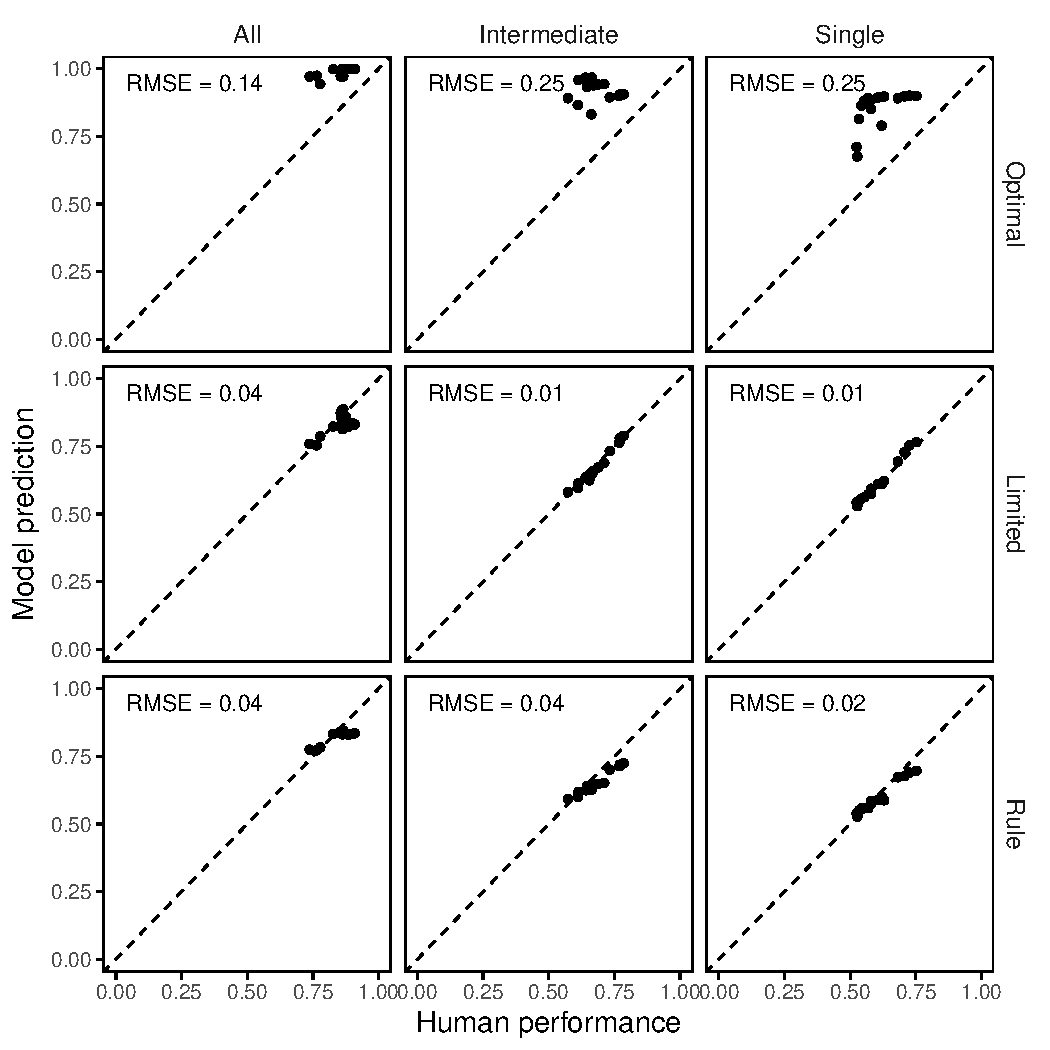
\includegraphics[width=0.7\textwidth]{figures/human-model-correlation-experiment-one.pdf}
    \caption{\small{\textbf{Scatterplot comparing the predictions of the three computational models to human performance in Experiment One.} Each panel contains a dot for the performance at each block and across all \textit{Dimensionality} conditions. Our results show that the \textsc{optimal} model consistently overestimates performance, while both the \textsc{limited} and \textsc{rule} models both closely match human performance across the different conditions in Experiment One.}}
  \label{model-comparison-experiment-one}
  \end{center}
\end{figure}

\begin{figure}[h!]
  \begin{center}
    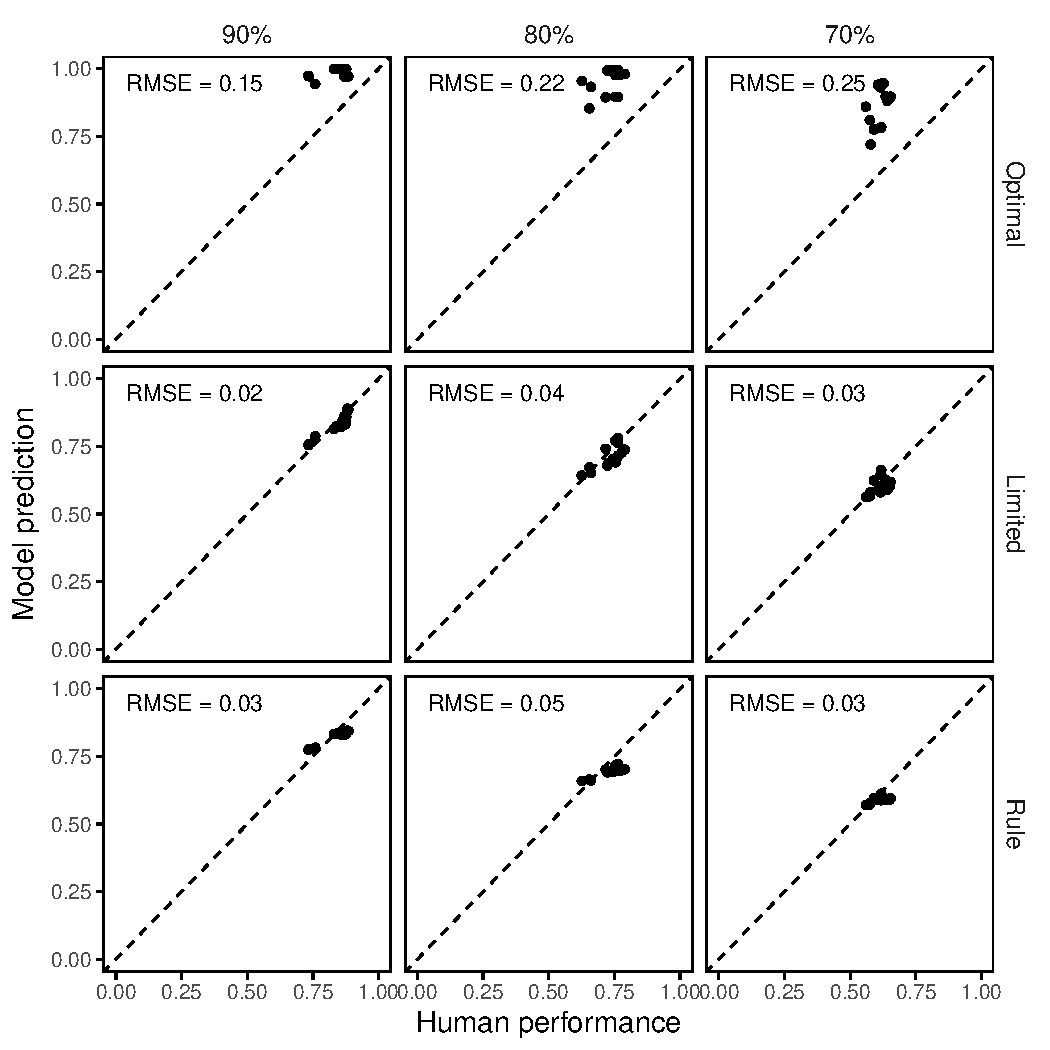
\includegraphics[width=0.7\textwidth]{figures/human-model-correlation-experiment-two.pdf}
    \caption{\small{\textbf{Scatterplot comparing the predictions of the three computational models to human performance in Experiment Two.} Each panel contains a dot for the performance at each block and across all \textit{Dimensionality} conditions.} Similar to the scatterplot in  Figure~\ref{model-comparison-experiment-one}, we find that the \textsc{optimal} model performs far better than humans on this task, while both the \textsc{limited} and \textsc{rule} models both track human performance closely.}
  \label{model-comparison-experiment-two}
  \end{center}
\end{figure}

Figures~\ref{model-comparison-experiment-one} and \ref{model-comparison-experiment-two} shows the correlation between human performance and the predictions from each of the three models across each condition. There are a number of observations we can make based on the different scatterplots shown here. First, the results show that the \textsc{optimal} model consistently outperforms humans in all conditions. While this provides a theoretical upper bound for how well people could do in the task, the results show that this limit was not attained in any of the conditions.

Second, both figures demonstrate that the predictions from both the \textsc{limited} and \textsc{rule} models fit reasonably well to the human data. In some of the conditions, they both appear to underpredict human performance, but they nevertheless capture the main qualitative patterns across both experiments. In particular, when categories are not family resemblance structures, both models predict that more features should hurt performance, and when the category structure is family resemblance based, both models predict that additional features should make no difference. Since this behavior precisely matches the qualitative pattern shown by people, it is perhaps no surprise that the \textsc{rule} and \textsc{limited} models provide a strong quantitative fit to human performance.

Perhaps somewhat disconcertingly, neither the quantitative nor the qualitative fits give compelling reason to prefer either the \textsc{rule} or \textsc{limited} model over each other. That said, it is important to realise that this analysis so far reflects \textit{aggregate} data: how well each model predicts the overall population average amongst our participants. Yet we know that population averages may be highly misleading when the goal is to infer what kinds of individual processes give rise to the behavior in question.
% For instance, if a population was actually made of two very different kinds of people, the aggregate might bear no resemblance to the behavior of any of the individuals involved.

\begin{figure}
	\centering
    \captionsetup[subfigure]{justification=centering}
    \begin{subfigure}[b]{0.45\textwidth}

      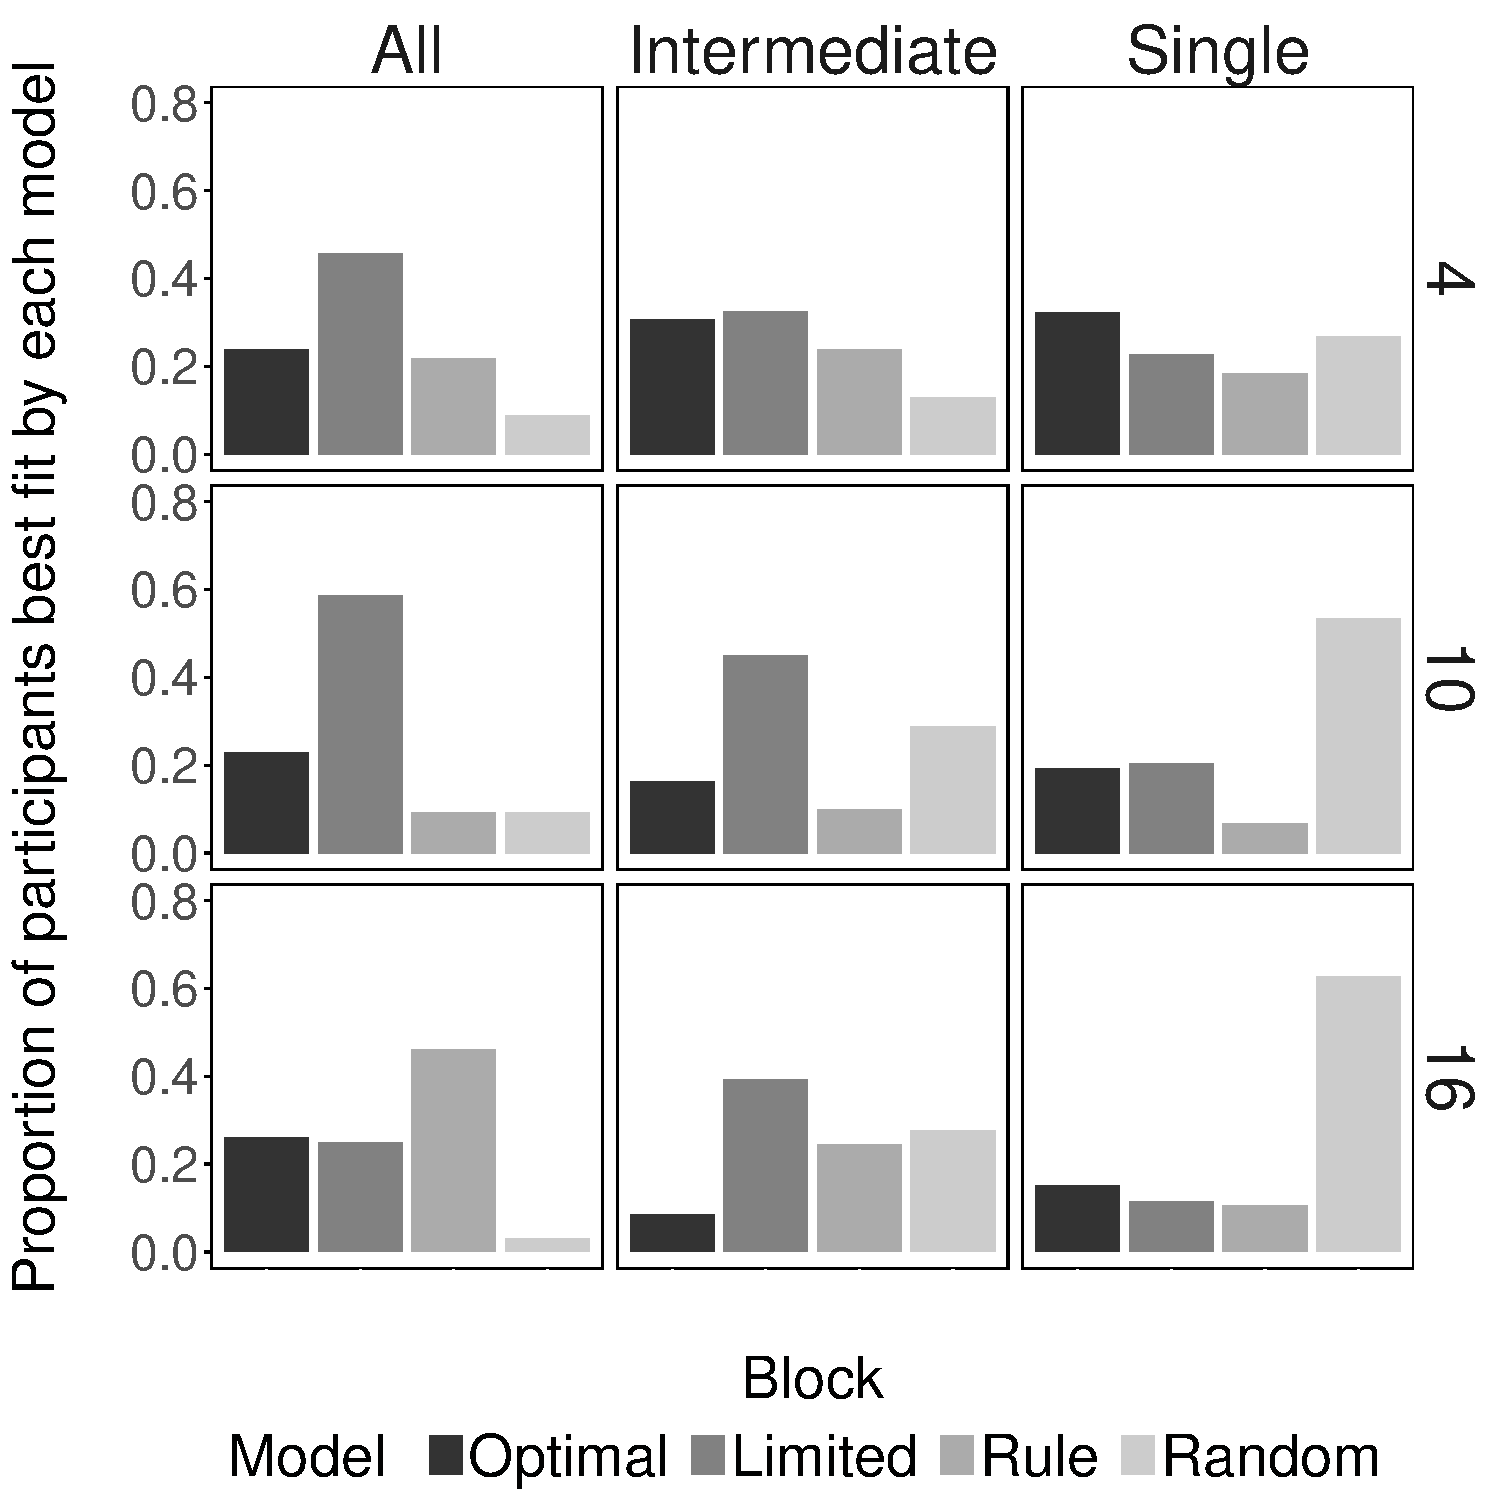
\includegraphics[width=\textwidth]{figures/individual-model-prop-by-structure-and-dim-experiment-one.pdf}
      \caption{Experiment 1}
    \end{subfigure}
    ~
    \begin{subfigure}[b]{0.45\textwidth}
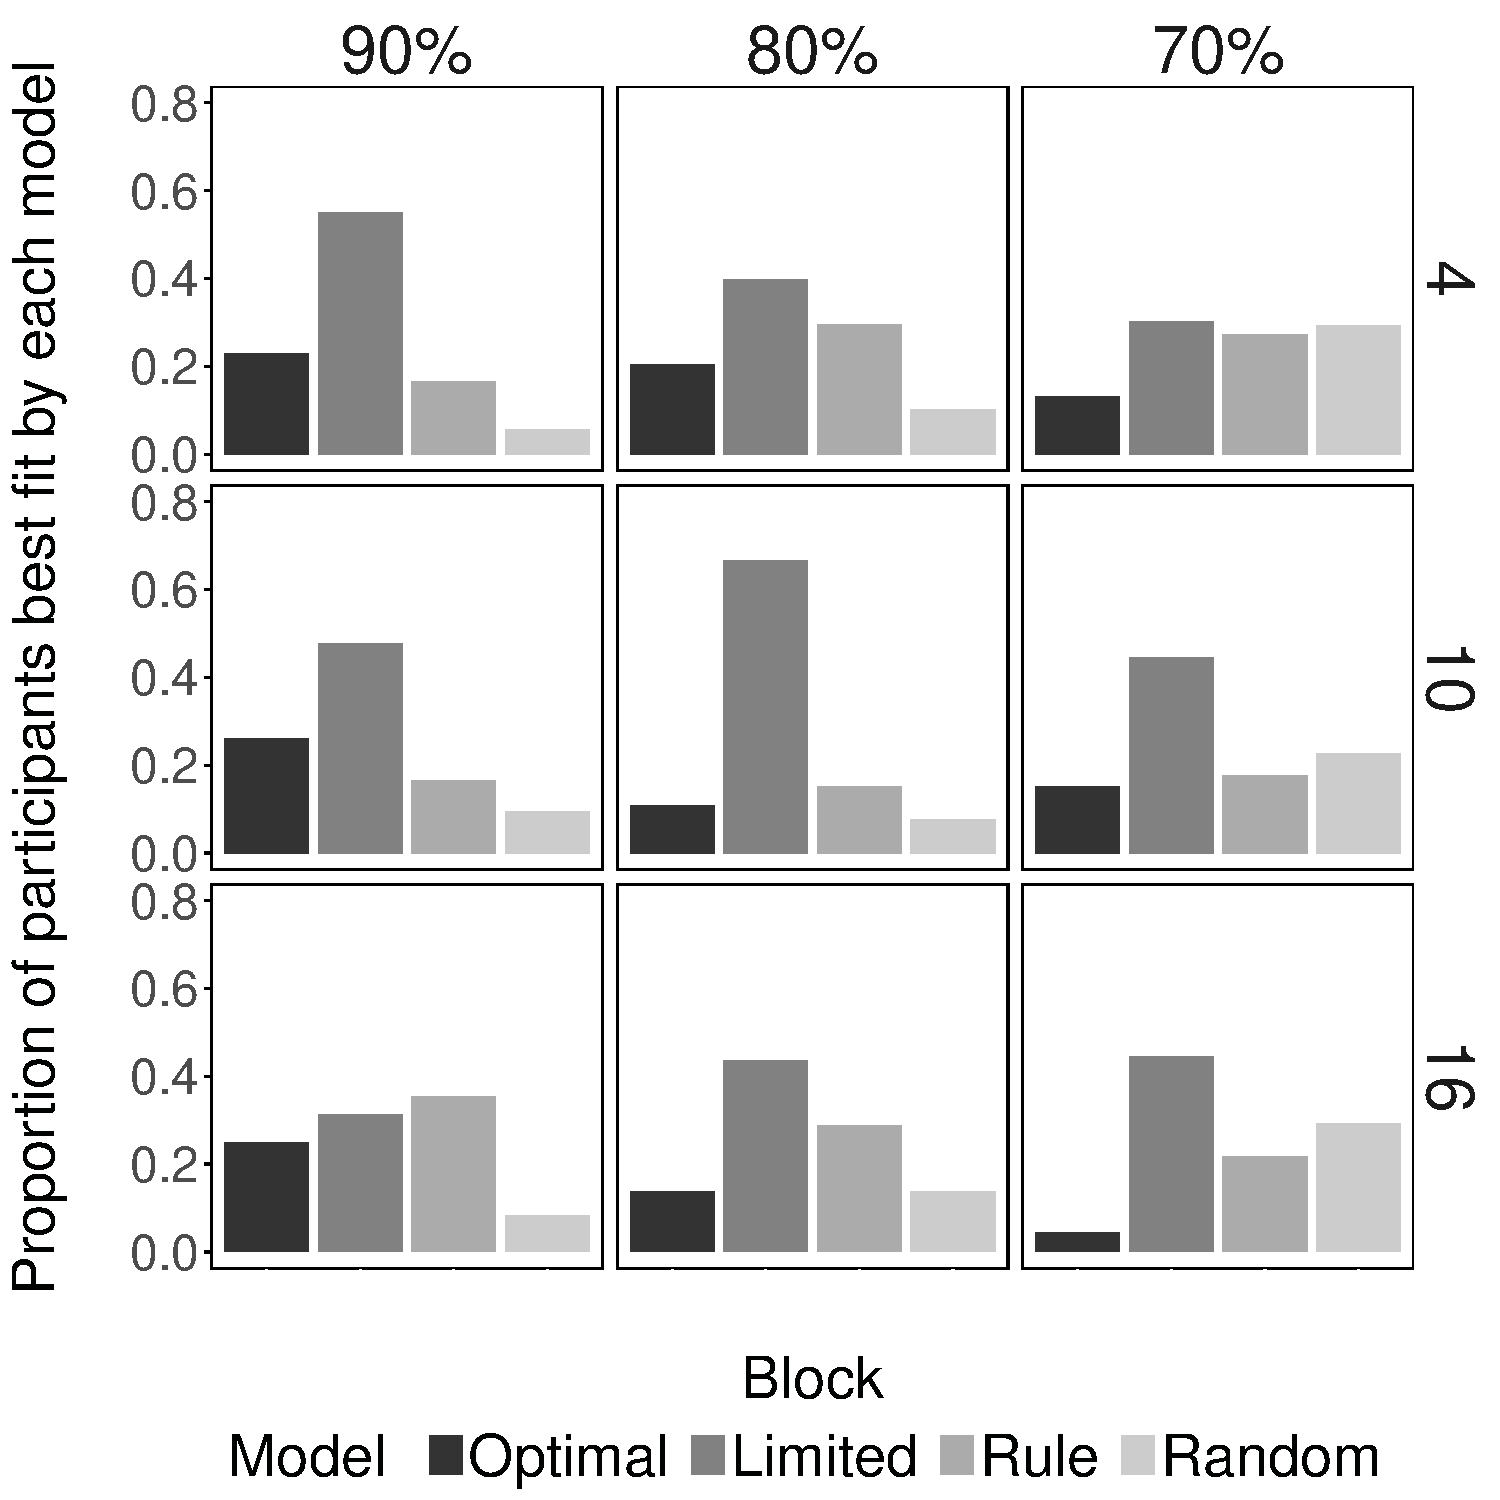
\includegraphics[width=\textwidth]{figures/individual-model-prop-by-structure-and-dim-experiment-two.pdf}
      \caption{Experiment 2}
    \end{subfigure}
    \vspace{3mm}
    \caption{\small{\textbf{Proportion of individuals who are best fit by each of the models in both experiments.} For each individual, we calculated the RMSE between their performance and each of the computational models, and assigned them to the model whose predictions led to the smallest RMSE. Across most of the conditions in both experiments, most people's pattern of performance most closely matched the predictions of the \textsc{limited} model, and not the \textsc{rule} model, despite the predictions of both models being very similar in the aggregate. The main exception to this pattern is in the more difficult conditions like the \textsc{single} category structure, in which a model consistent with random guessing did the best.}}
    \label{individual-fits}
\end{figure}

For this reason we also calculated which model best fit each of the individuals in each of the experiments (as reflected in the RMSE between each individual's accuracy and the model predictions from the same experimental condition as the individual), as shown in Figure~\ref{individual-fits}. A random guessing model was also included in the set of models, where the performance for each block was set at chance level (50\%). Although there is substantial variation across people, in the majority of conditions most people's performance best matches the \textsc{limited} model. The only exception is that in the most difficult conditions a substantial number are best fit by the \textsc{random} model, suggesting these participants were unable to learn the task. The \textsc{optimal} model describes performance the least well of the three theoretically motivated models.

\section{Discussion}

The term ``curse of dimensionality'' has been applied to a range of problems in machine learning, statistics and engineering, all of which share the common property that the space of possible solutions to an inference problem grows extraordinarily rapidly as the dimensionality increases. The same phenomenon applies to human category learning, and our goal in this paper has been to explore how the curse plays out for human learners.

At an empirical level we observed a clear pattern in which the curse of dimensionality is strongly moderated by the structure of the categories that need to be learned. Categories like those in the \textsc{single} condition, in which only a small number of features are relevant for predicting category membership, are heavily affected by dimensionality because the search problem (identifying the predictive feature) becomes harder as more irrelevant features are added. In contrast, the number of features does not appear to affect learning for family resemblance categories in which all features are somewhat predictive of category membership. A comparison of several computational models indicates that people's individual performance is best explained by model where learning and decision-making both proceed based on one feature at a time. This pattern was observed across the different category structures we tested, suggesting that people were not using different learning approaches to different category structures. Additionally, this result is consistent with theories of category learning that begin with single features that can be combined later on, such as Combination Theory \cite{wills2015combination}, rather than beginning from the overall stimulus and dividing it into distinct attributes.

% WK: previous version of the final sentence in the paragraph above
% Comparing our results to an ideal observer model that could attain the highest possible performance, we find numerous instances in which people's behaviour deviates from the model's predictions and suggests that people may be employing a different strategy to learn the categories.

% WK: I decided against putting these paragraphs back in, it's a very minor point and I'm not sure how much it adds
% There are some interesting nuances within this fairly straightforward picture. Although the failure of the \textsc{optimal} model to predict human performance was robust in both experiments as well as the individual-level analysis, the distinction between the \textsc{rule} and \textsc{limited} model is less evident: they did similarly well in predicting aggregate performance, and only in individual-level analyses did the \textsc{limited} model show an improvement. Why?

% In some ways the similar performance between the \textsc{rule} and \textsc{limited} models should be no surprise, because they are very similar models. Both are based on a decision rule that uses a single feature, and both only update the representation for that single feature on each trial. The difference between the two stems from the difference in representation: the \textsc{limited} model learns about the category predictiveness of a stimulus feature dimension (a location on the stimuli that can take multiple feature values), while the \textsc{rule} model learns about a single stimulus value (the specific stimulus feature in a location).
% Put another way, both models pay attention only to one feature on any given trial. However, the \textsc{limited} model updates $p(y|\textbf{x})$ according to Equation~\ref{limited-prototype-eq} which contains information about both feature \textit{values}. By contrast, the \textsc{rule}  model learns about each feature value independently, resulting in a hypothesis space that consists of $2N$ different rules, two for each feature. This means that for the \textsc{rule} model, choosing to discard the rule: \texttt{if value 0 on feature K, choose category A} says nothing about the validity of the rule: \texttt{if value 1 on feature K, choose category A}.

% The consequence of this is that the \textsc{limited} model can learn somewhat faster than the \textsc{rule} model. It also tends to gradually improve throughout training, rather than plateauing sooner in training, probably because abstracting over feature dimensions rather than learning specific feature values in isolation provides a learning benefit. On an individual level, this is the pattern people tended to show.
% This subtle difference accords with other research finding that abstracting across feature values fits people better than a hypothesis-testing model that did not \cite{gershman2010learning, niv2015reinforcement}.

One of the main conclusions from this work is that it is not very meaningful to discuss the effect of dimensionality without considering what kind of category structure is being learned, that is, both the number and nature of the features and how predictive each feature is of category membership. In fact, the role of category structure may help explain away apparent differences in the literature. For instance, previous research indicating that additional features hurt performance used features that were not predictive of category membership \cite{bourne1959mathematical, edgell1996irrelevant}, consistent with our \textsc{single} condition in Experiment 1. Other studies that found that adding features did not have any effect used family resemblance categories, consistent with the \textsc{all} conditions in both of our experiments  (\citeA{hoffman2006category} Experiments 1 and 2, \citeA{minda2001prototypes} Experiment 4, \citeA{hoffman2008prior} Experiment 1). There were only two results we were not able to replicate, both reflecting an improvement in learning with more features (\citeA{hoffman2006category} Experiment 3 and \citeA{minda2001prototypes} Experiment 1). However, in both of those studies, other aspects of category structure covaried with the number of features, providing an alternate explanation for results that differed from ours. For instance, in Experiment 1 of \citeA{minda2001prototypes}, the categories with fewer features were less structured, and when this confound was addressed in Experiment 4 of that paper, the effect went away.

Our computational work explains how these apparently qualitatively different effects for different kinds of categories can all emerge parsimoniously from one unified model. A model with limited capacity predicts that additional features should neither hurt nor help in categories with family resemblance structure, since subsequent features provide the same amount of information as existing ones. However, the same limited-capacity model should struggle in more rule-based categories, when learning involves searching over the space of features to identify the (few) predictive ones. The effect only occurs for a learner who is limited enough in capacity that they cannot simultaneously learn over all features at once.

One limitation of this work concerns the nature of the stimulus generation process. As the stimuli were generated by first selecting the category label, and selecting the features conditional on the category label, more stimuli may have been selected that were closer to the prototype in the \textsc{all} condition rather than the \textsc{single} condition in Experiment One, leading to a biased distribution of stimuli, favouring stimuli that are easier to classify in the \textsc{all} condition. Was the improved performance in the \textsc{all} condition a result of this? In order to address this possibility, we conducted an analysis of performance as a function of likelihood of generation. While fewer stimuli away from the prototype were indeed generated in the \textsc{all} condition, performance on the trials involving these stimuli were better than equivalent stimuli from the \textsc{single} category structure, and more so in cases where there were additional relevant features. The Appendix contains further details.

\subsection{Broader implications for human learning}

The fact that human learning deviates systematically from the \textsc{optimal} model is theoretically interesting and highlights an important difference between real world learning and many category learning experiments. Both our experiments had features with \textit{class-conditional independence}, in which the stimulus features are conditionally independent of one another as long as one knows the category to which the stimulus belongs. This assumption does not hold in general, but in some situations it might provide a reasonable first approximation. Indeed, people do appear to assume class-conditional independence, at least at first, in some category-learning tasks \cite{jareckietalinpress}.

However, from a computational modeling perspective, it is important to recognize the limitations that this assumption imposes: the reason that our ideal observer model is able to perform \textit{better} on family resemblance categories as the number of features increases is that it exploits the fact that every additional feature conveys independent information about the category. When class-conditional independence holds, family resemblance categories become easier to learn as the dimensionality increases. This does \textit{not} match the pattern we observed in our data, in which people's performance on family resemblance categories was the same regardless of the number of features in the stimuli.

Instead, the pattern of learning in these tasks is more accurately predicted by a capacity limited model that only processes a modest amount of information on each trial. However, the reason why people only process a limited amount of information is not clear. One possible interpretation is that memory limitations may restrict how people are able to encode these novel stimuli in memory or reason about the relationship between features and category labels. Depending on the relationship among features and between them and category labels, in real life one might end up making better categorization decisions by using a limited number of predictive features rather than attempting to process all information inherent in the stimuli. In other words, human learners might differ from our optimal statistical learning model not because of the limits of human cognition but because human cognition is shaped by an environment in which class conditional independence is a poor assumption, and that human learners are better described by other kinds of inductive biases.

% One possible explanation is that is that the class-conditional independence structure in our experiments does not match the true relationship between features and categories for most categories the world. If that is the case, it would imply that perhaps people are adaptive by relying on a single or small set of features when learning categories. Depending on the relationship among features and between them and category labels, in real life one might end up making better categorization decisions by using a limited number of predictive features rather than attempting to process all information inherent in the stimuli. In other words, human learners might differ from our optimal statistical learning model not because of the limits of human cognition but because human cognition is shaped by an environment in which class conditional independence is a poor assumption, and that human learners are better described by other kinds of inductive biases.

% TODO: add potential discussion paragrpah about dual process models as suggested by reviewers?

% TODO: commented out in previous version, ignore
% That being said, it is clear that human category learning must impose \textit{some} biases. As we saw, when stimuli are described in terms of $N$ binary valued features, there are $2^N$ logically distinct stimuli that a learner might be asked to classify and $2^{2^N}$ possible ways to assign stimuli to two categories. In our experiments, when the amoeba were described using four different features the stimulus space consists of 16 distinct stimuli. During the course of a 100 trial experiment participants will almost certainly observe all 16 stimuli many times. It is quite possible to solve this problem by a pure exemplar memorization strategy: no inductive bias is required other than the (modest) assumption that category labels do not change over time.

% In the conditions with 16 features, however, exemplar memorization is not sufficient to achieve acceptable performance. In it there are 65,536 logically distinct \textit{stimuli} and approximately $2\times 10^{19728}$ possible ways to sort these items into two categories. This means that the learner will have observed no more than 0.15\% of the items during the course of a 100-trial experiment. Regardless of the particulars of how it is achieved, classifying novel items at a 90\% accuracy level when only a tiny proportion of the stimuli have been observed requires a strong inductive bias of some kind.

% TODO: add back in references to limited model?
The question of what other inductive biases are required to explain how humans are affected by the curse of dimensionality in some cases and not others is beyond the scope of this paper, but we can speculate about possible answers. One possibility is an inductive bias for sparsity \cite{gershman2010learning}, which assumes that only one (or a limited) number of features is relevant for categorization. Thus, the relevant features for this task could be learned through selective attention, a process where attentional weights for particular features increase or decrease based on their ability to make correct classification decisions. This kind of approach has been successfully employed by a number of existing models of categorization to explain other patterns in human category learning \cite{nosofsky1986attention, kruschke1992alcove}, and is a potential future avenue of exploration for a richer explanation of how people learn categories with many features.

% TODO: commented out in previous version, ignore
% This is reminiscent not only of fast and frugal models of decision making \cite{gigerenzer1999simple}, but is also somewhat akin to sequential sampling models used in simple decision-making \cite{ratcliff1978theory,brown2008simplest,vickers1979decision,luce1986response}. The sequential sampling framework is especially appealing insofar as it has previously been applied to a variety of problems in complex decision making \cite{lee2004evidence,newell2011right,navarro2016learning} including classification \cite{nosofsky1994rule}, and has strong connections to statistical decision making \cite{wald1947foundations,vul2014one}.

A second, alternative approach towards lifting the curse dimensionality is to reduce the number of features that are represented or encoded in the first place. Such methods focus on reducing the number of dimensions via manifold learning \cite{tenenbaum1998mapping} or using structured representations \cite{kemp2009structured, tenenbaum2011grow, lake2015human}. These kinds of approaches have been pursued with considerable success in semantic representation \cite{griffiths2007topics,landauerdumais97}. It is, of course, possible that human learning is versatile enough to incorporate the fundamental insights from both exploiting limited memory and attentional capacities and reducing the effective dimensionality of incoming stimuli. Pursuing these issues further is a matter for future work.

\section{Acknowledgments}

Research costs were supported by grants from the Australian Research Council (DP110104949 and DP150103280). AP received salary support from DE12010378 and AH was supported by  DP110104949 and DP150103280.

\bibliographystyle{apacite}
\bibliography{references}

\section{Appendix}

The Discussion referred to an additional analysis comparing performance in the \textsc{all} and \textsc{single} conditions as a function of the likelihood of generating each stimulus. It is evident from Figure~\ref{fig:stimulus-distribution} that classification performance on the same stimuli (with the same likelihood of being generated) was higher in the \textsc{all} than in the \textsc{single} condition.

\begin{figure}[h!]
  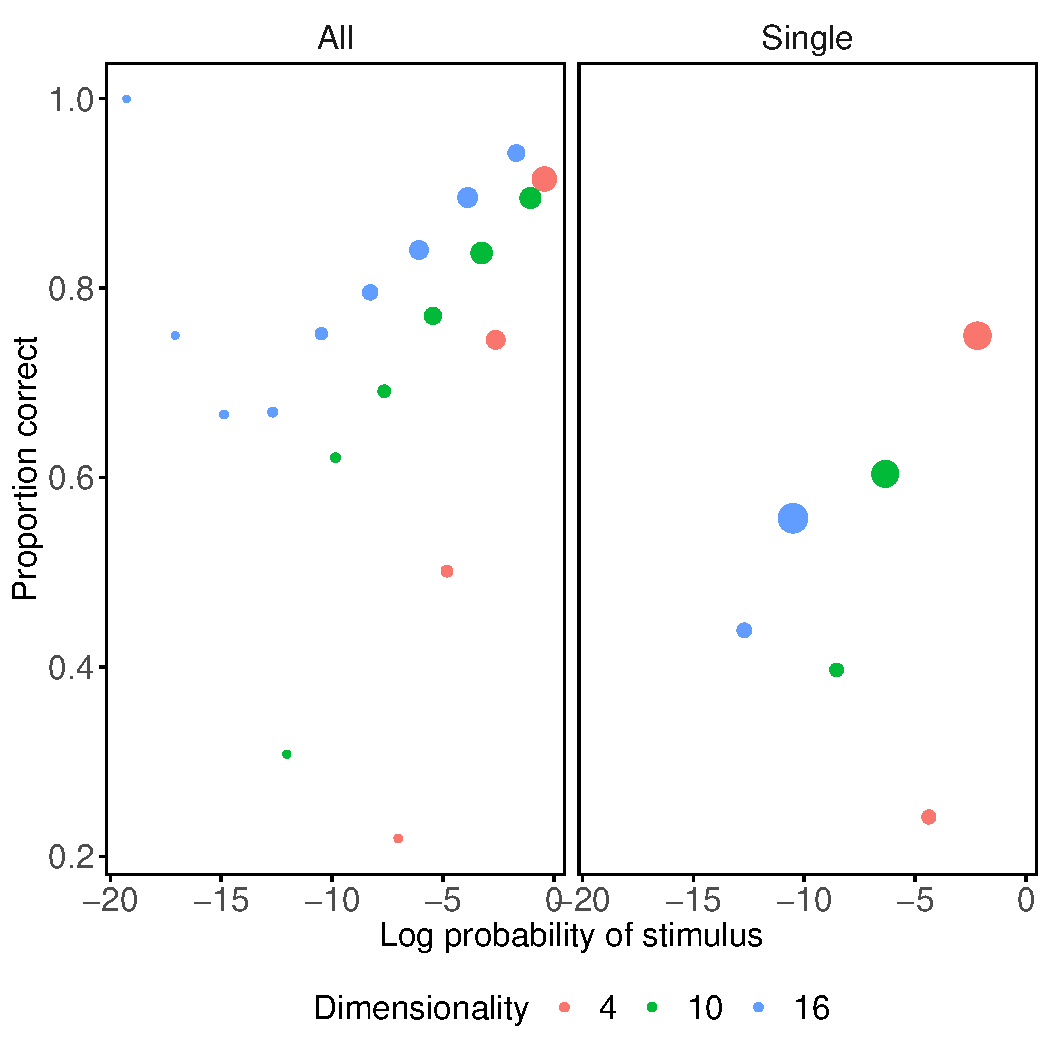
\includegraphics[width=0.9\linewidth]{figures/stim-prob-performance.pdf}
  \caption{Comparison of the log probability of stimuli vs. classification performance in the \textsc{all} vs. \textsc{single} category structures in Experiment One. The log probabilities were calculated by the likelihood of generating the particular stimuli under each of the two category structures, with smaller values indicating less likely stimuli. We see that fewer stimuli in the \textsc{all} category structure are sampled away from the prototype, but classification performance remains high, and more so with additional relevant features.}
  \label{fig:stimulus-distribution}
\end{figure}



% TODO: put this text at the very end of the article, not needed anyore

% WK: this paragraph was pretty strong, and feels too easy to be called out by reviewers
% While both the \textsc{rule} and \textsc{limited} models better account for the performance of humans at the aggregate and individual levels much better than the \textsc{optimal} model, when interpreting them as process models they make a number of strong assumptions that are weaker than what humans seem to be doing. For example, in the \textsc{limited} model it only updates and decides using a single feature on any given trial, but other research in category learning suggests that people can combine information from more than a single feature to make judgments \cite{gluck2002people}. Thus, this reduces the plausibility that the \textsc{limited} model is a complete process-level description of people's behaviour in this task, and that further work is necessary.

% We begin by looking at the predictions of the ideal observer model across both tasks. Figure~\ref{optimal-model-comparison-experiment-one} (top row) shows that for Experiment One, the model predicts that performance is highest in the \textsc{all} category structure, followed by the \textsc{intermediate} structure, with the worst performance in the \textsc{single} structure. Similarly, as Figure~\ref{optimal-model-comparison-experiment-two} (top row) reveals, the model predicts the best performance in the 90\% condition and the least in the 70\% condition.

% However, despite human performance matching the qualitative trends as predicted by the \textsc{optimal} model across \textit{Structure} for Experiment One, and \textit{Predictiveness} for Experiment Two, the predictions of the \textsc{optimal} model deviate from human performance in a number of ways. This is illustrated in the panels on the bottom rows of Figures~\ref{optimal-model-comparison-experiment-one} and ~\ref{optimal-model-comparison-experiment-two}, where the difference between the model predictions and human performance are plotted. First, the \textsc{optimal} model consistently predicts that performance should be far higher than what we empirically observe, as the difference between the model predictions and human performance is above zero for every condition. Second, for all of the conditions where additional features are helpful for categorization, the model shows increasing performance for additional features. On the other hand, for humans the effect of additional features hurts performance when most of the features are weakly predictive (like the \textsc{intermediate} structure from Experiment 1), or that performance stays the same (as observed for all of the family resemblance structures). In addition, for the \textsc{single} condition in Experiment One where additional features are not informative, humans show decreasing performance for more features, whereas the ideal observer model predicts that by the end of the experiment should result in equal performance across the \textit{Dimensionality} conditions. This analysis highlights that human behaviour is far from the maximum performance that is achievable as demonstrated by the ideal observer model. We discuss possibilities on how computational models could explain this pattern of results in the discussion section.

% TODO: integrate previous model results with this one
% \subsection{Model results}

% Similar to the results obtained for the  \textsc{optimal} model, we simulated the \textsc{rule} and \textsc{limited} models 10,000 times for each of the experimental conditions in both experiments, where each simulation mimicked a 100-trial experiment. On each trial, a new stimulus was generated in exactly the same manner as the experiment, the model then made a prediction of the category label, and then received feedback and updated its category representations. The full set of results comparing human performance to all three models are shown in Figures~\ref{model-comparison-experiment-one} and \ref{model-comparison-experiment-two}.

% \begin{table}[t]
% \centering
% \begin{tabular}{l|c|c|}
% \cline{2-3}
% & \multicolumn{1}{l|}{Experiment 1} & \multicolumn{1}{l|}{Experiment 2} \\ \hline
% \multicolumn{1}{|l|}{Optimal}  & 0.228  & 0.217                               \\ \hline
% \multicolumn{1}{|l|}{Limited} & 0.038 & \textbf{0.028}                      \\ \hline
% \multicolumn{1}{|l|}{Rule} & \textbf{0.029}   & 0.037                               \\ \hline
% \multicolumn{1}{|l|}{Random} & 0.237   & 0.251                               \\ \hline
% \end{tabular}
% \caption{\small{\textbf{Error estimates between model predictions and human performance.} Errors are root-mean-squared error (RMSE) between the aggregate model predictions of accuracy and the aggregate human accuracy. In both experiments, the \textsc{limited} and \textsc{rule} models fit far better than the \textsc{optimal} model and a \textsc{random} model that guesses on each trial, although which of the two has the best fit changes from Experiment 1 to 2.}}
% \label{table-rmse}
% \end{table}

% How do the predictions of the \textsc{rule} and \textsc{limited} model differ from the \textsc{optimal} model? Similar to the analyses in the main body of this Chapter, I begin by looking at aggregate performance across participants. Similar to the \textsc{optimal} model, both the \textsc{rule} and \textsc{limited} models produce the main qualitative patterns shown in the participant data across both experiments. However, where the \textsc{optimal} model failed to capture the quantitative aspects of human performance, both the \textsc{rule} and \textsc{limited} models do a better job. In particular, when categories are not family resemblance structures, more features should hurt performance, and when the category structure is family resemblance based, additional features should make no difference. Since this behavior precisely matches the qualitative pattern shown by people, it is perhaps no surprise that the \textsc{rule} and \textsc{limited} models quantitatively fit human performance far better (see Table~\ref{table-rmse}).

% Perhaps somewhat disconcertingly, neither the quantitative nor the qualitative fits give compelling reason to prefer either the \textsc{rule} or \textsc{limited} model over each other. That said, it is important to realise that this analysis so far reflects \textit{aggregate} data: how well each model predicts the overall population average amongst our participants. Yet we know that population averages may be highly misleading when the goal is to infer what kinds of individual processes give rise to the behavior in question. For instance, if a population was actually made of two very different kinds of people, the aggregate might bear no resemblance to the behavior of any of the individuals involved.

% \begin{figure}
% 	\centering
%     \captionsetup[subfigure]{justification=centering}
%     \begin{subfigure}[b]{0.45\textwidth}
%             \caption{Experiment 1}
%     	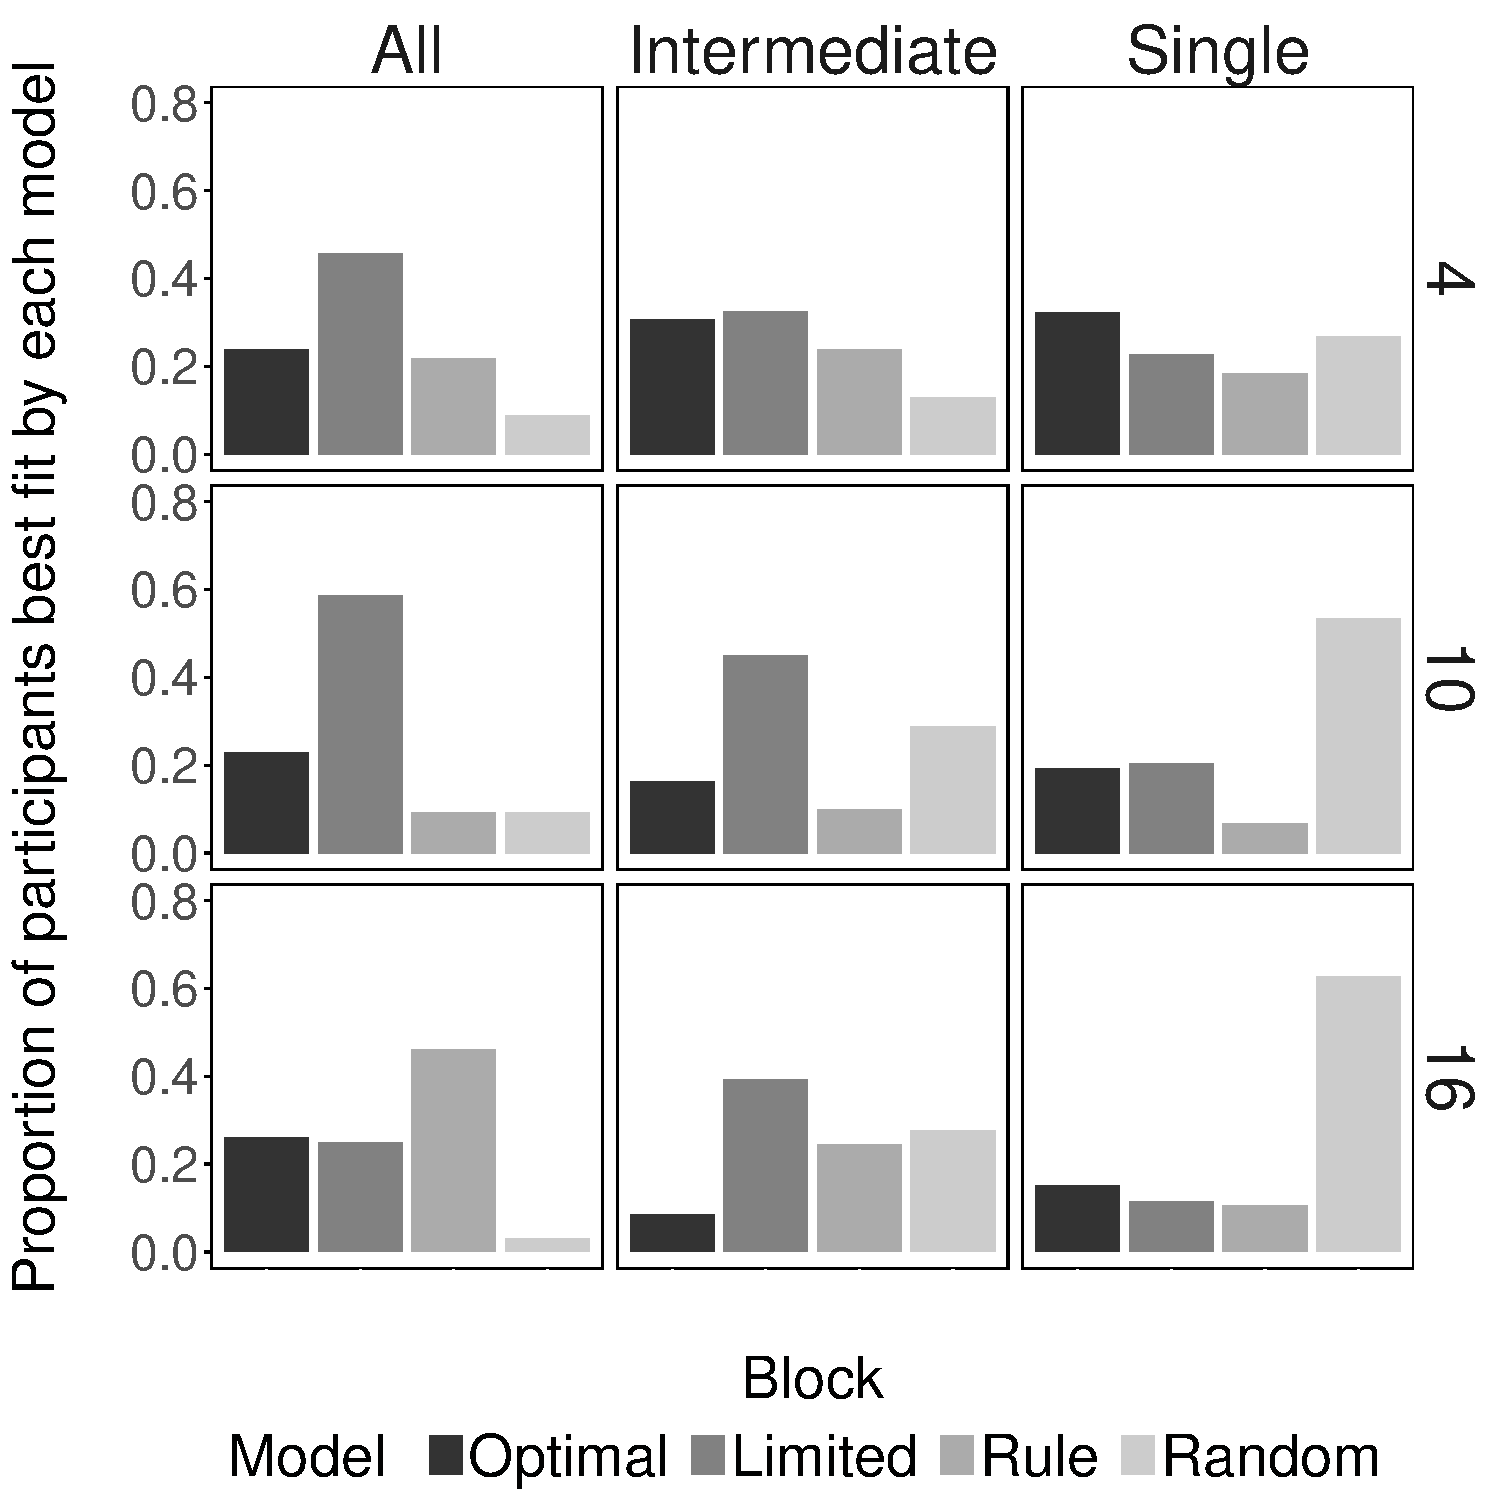
\includegraphics[width=\textwidth]{figures/individual-model-prop-by-structure-and-dim-experiment-one.pdf}
%     \end{subfigure}
%     ~
%     \begin{subfigure}[b]{0.45\textwidth}
%             \caption{Experiment 2}
% 		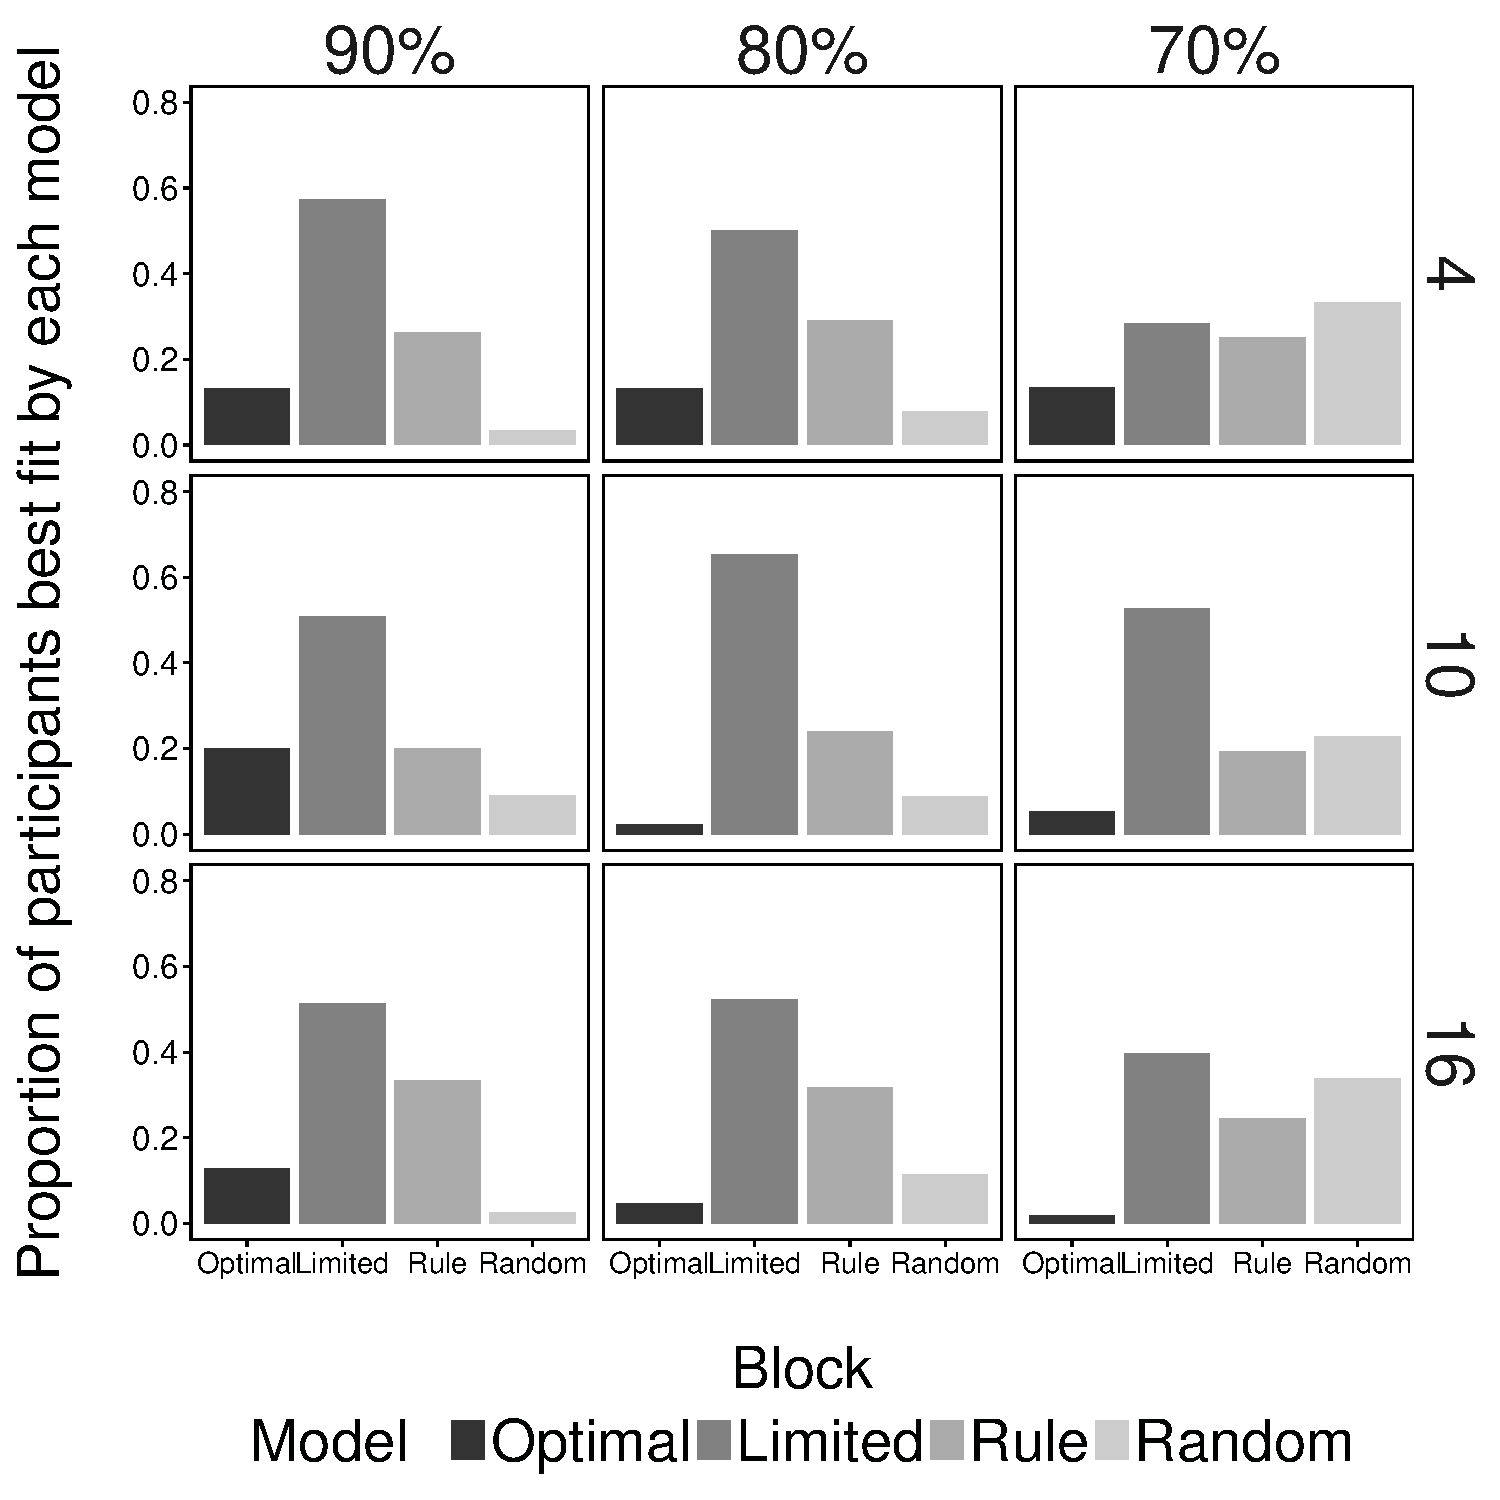
\includegraphics[width=\textwidth]{figures/individual-model-prop-by-coherence-and-dim-experiment-two.pdf}
%     \end{subfigure}
%     \vspace{3mm}
%     \caption{\small{\textbf{Proportion of individuals who are best fit by each of the models in both experiments.} Most of the time, most people's pattern of performance most closely matched the predictions of the \textsc{limited} model. The main exception is in the more difficult conditions like the \textsc{single} category structure, in which a model consistent with random guessing did the best.}}
%     \label{individual-fits}
% \end{figure}

% For this reason we also calculated which model best fit each of the individuals in each of the experiments (as reflected in the RMSE between each individual's accuracy and the model predictions from the same experimental condition as the individual), as shown in Figure~\ref{individual-fits}. It is evident that although there is substantial variation across people, in the majority of conditions most people are best fit by the \textsc{limited} model. The only exception is that in the most difficult conditions a substantial number are best fit by a model that guesses randomly, suggesting these participants were unable to learn the task. The \textsc{optimal} model describes performance the least well of the three theoretically motivated models.

% While both the \textsc{rule} and \textsc{limited} models better account for the performance of humans at the aggregate and individual levels much better than the \textsc{optimal} model, when interpreting them as process models they make a number of strong assumptions that are weaker than what humans seem to be doing. For example, in the \textsc{limited} model it only updates and decides using a single feature on any given trial, but other research in category learning suggests that people can combine information from more than a single feature to make judgments \cite{gluck2002people}. Thus, this reduces the plausibility that the \textsc{limited} model is a complete process-level description of people's behaviour in this task, and that further work is necessary.


\end{document}

%%% Local Variables:
%%% mode: latex
%%% TeX-master: t
%%% End:

